%Version 2.1 April 2023
% See section 11 of the User Manual for version history
%
%%%%%%%%%%%%%%%%%%%%%%%%%%%%%%%%%%%%%%%%%%%%%%%%%%%%%%%%%%%%%%%%%%%%%%
%%                                                                 %%
%% Please do not use \input{...} to include other tex files.       %%
%% Submit your LaTeX manuscript as one .tex document.              %%
%%                                                                 %%
%% All additional figures and files should be attached             %%
%% separately and not embedded in the \TeX\ document itself.       %%
%%                                                                 %%
%%%%%%%%%%%%%%%%%%%%%%%%%%%%%%%%%%%%%%%%%%%%%%%%%%%%%%%%%%%%%%%%%%%%%

%%\documentclass[referee,sn-basic]{sn-jnl}% referee option is meant for double line spacing

%%=======================================================%%
%% to print line numbers in the margin use lineno option %%
%%=======================================================%%

%%\documentclass[lineno,sn-basic]{sn-jnl}% Basic Springer Nature Reference Style/Chemistry Reference Style

%%======================================================%%
%% to compile with pdflatex/xelatex use pdflatex option %%
%%======================================================%%

%%\documentclass[pdflatex,sn-basic]{sn-jnl}% Basic Springer Nature Reference Style/Chemistry Reference Style


%%Note: the following reference styles support Namedate and Numbered referencing. By default the style follows the most common style. To switch between the options you can add or remove “Numbered” in the optional parenthesis. 
%%The option is available for: sn-basic.bst, sn-vancouver.bst, sn-chicago.bst, sn-mathphys.bst. %  
 
%%\documentclass[sn-nature]{sn-jnl}% Style for submissions to Nature Portfolio journals
%%\documentclass[sn-basic]{sn-jnl}% Basic Springer Nature Reference Style/Chemistry Reference Style
\documentclass[sn-mathphys,Numbered]{sn-jnl}% Math and Physical Sciences Reference Style
%%\documentclass[sn-aps]{sn-jnl}% American Physical Society (APS) Reference Style
%%\documentclass[sn-vancouver,Numbered]{sn-jnl}% Vancouver Reference Style
%%\documentclass[sn-apa]{sn-jnl}% APA Reference Style 
%%\documentclass[sn-chicago]{sn-jnl}% Chicago-based Humanities Reference Style
%%\documentclass[default]{sn-jnl}% Default
%%\documentclass[default,iicol]{sn-jnl}% Default with double column layout

%%%% Standard Packages
%%<additional latex packages if required can be included here>

\usepackage{graphicx}%
\usepackage{multirow}%
\usepackage{amsmath,amssymb,amsfonts}%
\usepackage{amsthm}%
\usepackage{mathrsfs}%
\usepackage[title]{appendix}%
\usepackage{xcolor}%
\usepackage{textcomp}%
\usepackage{manyfoot}%
\usepackage{booktabs}%
\usepackage{algorithm}%
\usepackage{algorithmicx}%
\usepackage{algpseudocode}%
\usepackage{listings}%
\usepackage{graphicx}
\usepackage{url}
\usepackage{breakurl}
\usepackage{hyperref}
\usepackage{xurl}
%%%%

%%%%%=============================================================================%%%%
%%%%  Remarks: This template is provided to aid authors with the preparation
%%%%  of original research articles intended for submission to journals published 
%%%%  by Springer Nature. The guidance has been prepared in partnership with 
%%%%  production teams to conform to Springer Nature technical requirements. 
%%%%  Editorial and presentation requirements differ among journal portfolios and 
%%%%  research disciplines. You may find sections in this template are irrelevant 
%%%%  to your work and are empowered to omit any such section if allowed by the 
%%%%  journal you intend to submit to. The submission guidelines and policies 
%%%%  of the journal take precedence. A detailed User Manual is available in the 
%%%%  template package for technical guidance.
%%%%%=============================================================================%%%%

%\jyear{2021}%

%% as per the requirement new theorem styles can be included as shown below
\theoremstyle{thmstyleone}%
\newtheorem{theorem}{Theorem}%  meant for continuous numbers
%%\newtheorem{theorem}{Theorem}[section]% meant for sectionwise numbers
%% optional argument [theorem] produces theorem numbering sequence instead of independent numbers for Proposition
\newtheorem{proposition}[theorem]{Proposition}% 
%%\newtheorem{proposition}{Proposition}% to get separate numbers for theorem and proposition etc.

\theoremstyle{thmstyletwo}%
\newtheorem{example}{Example}%
\newtheorem{remark}{Remark}%

\theoremstyle{thmstylethree}%
\newtheorem{definition}{Definition}%

\raggedbottom
%%\unnumbered% uncomment this for unnumbered level heads

\begin{document}

\title[Article Title]{
\centering
Supplementary Information for
\\
Energy-system interactions reshape offshore hydrogen trade and carbon mitigation in Europe
}

%%=============================================================%%
%% Prefix	-> \pfx{Dr}
%% GivenName	-> \fnm{Joergen W.}
%% Particle	-> \spfx{van der} -> surname prefix
%% FamilyName	-> \sur{Ploeg}
%% Suffix	-> \sfx{IV}
%% NatureName	-> \tanm{Poet Laureate} -> Title after name
%% Degrees	-> \dgr{MSc, PhD}
%% \author*[1,2]{\pfx{Dr} \fnm{Joergen W.} \spfx{van der} \sur{Ploeg} \sfx{IV} \tanm{Poet Laureate} 
%%                 \dgr{MSc, PhD}}\email{iauthor@gmail.com}
%%=============================================================%%

\author[1,2]{\fnm{Sheng} \sur{Wang}}\email{sheng.wang@newcastle.ac.uk}

\author[2,3]{\fnm{Muhammad} \sur{Maladoh Bah}}\email{muhammad.maladohbah@seai.ie}

% \author[4]{\fnm{Zeyuan} \sur{Xu}}\email{}


\affil*[1]{\orgdiv{School of Engineering}, \orgname{Newcastle University}, \orgaddress{\street{Newcastle University}, \city{Newcastle upon Tyne}, \postcode{NE17RU}, \country{The United Kingdom}}}

\affil[2]{\orgdiv{School of Electrical and Electronic Engineering}, \orgname{University College Dublin}, \orgaddress{\street{Belfield}, \city{Dublin}, \postcode{D04 V1W8}, \country{Ireland}}}

\affil[3]{ \orgname{Sustainable Energy Authority Of Ireland}, \orgaddress{\street{3 Park Place, Hatch Street}, \city{Dublin}, \postcode{D02 FX65}, \country{Ireland}}}

% \affil[4]{\orgdiv{Department of Chemical and Biomolecular Engineering}, \orgname{National University of Singapore}, \orgaddress{\city{Singapore}, \postcode{117585}, \country{Singapore}}}


\maketitle
\newpage
\tableofcontents
\newpage

\section{Introduction to the supplementary information}

This supplementary information illustrates the detailed models and data used in this paper. 
Section 2 introduces the wind resources in Ireland's marine areas, as well as physical models of offshore wind turbine arrays considering the impacts of the wake effect.
Section 3 developed frameworks to evaluate the levelized production cost for multiple offshore resource utilisation schemes, including electricity, liquefied hydrogen, and ammonia.
Using these data as inputs, Section 4 proposes a multi-energy systems (including power systems, and gas systems with hydrogen integration) optimisation framework to investigate the domestic integration potential of renewable electricity and green hydrogen from offshore wind. Three scenarios of offshore wind in 2030, 2040, and 2050, as outlined by the Irish government, are analysed. 
Based on the remaining capacity of hydrogen from domestic integration and cost-supply curves, Section 5 develops an international trading model to project the cross-border hydrogen trading landscape. Carbon mitigation is also analysed to highlight Ireland's contribution to reshaping Europe's net-zero transitions.

\section{Positioning of this study}

The main manuscript claims a first integrated European-scale assessment because the modelling chain combines components that are usually treated separately in the offshore hydrogen literature. Representative prior studies have quantified offshore wind-to-hydrogen production costs for Europe or individual regions, including North Sea, UK, Polish and Iberian cases \cite{rogeau2023techno, giampieri2024techno, komorowska2023evaluating, gonzalez2024techno, calado2024assessment}. European hydrogen infrastructure and demand studies have also assessed future cross-border demand, infrastructure corridors, and global import prospects \cite{EuropeanHydrogenBackbone, Analysingfuturedemand, IEAGlobalHydrogenReview2025, IEAGlobalHydrogenReviewTrade2025, IRENAGlobalHydrogenTradeOutlook2022}. These studies provide important inputs and benchmarks, but they do not jointly resolve how geospatial production costs, hourly domestic power-gas absorption, shipping-based hydrogen and ammonia exchange, external import competition, and supplier-specific carbon mitigation interact in one optimisation workflow.

\begin{table}[h]
\centering
\scriptsize
\setlength{\tabcolsep}{1pt}
\caption{Feature comparison between representative prior study types and the present integrated assessment. A check mark indicates that the feature is explicitly represented in the study type. A dash indicates that the feature is outside the main scope of that study type.}
\label{tab:novelty-comparison}
\begin{tabular}{p{2.8cm}p{1.4cm}p{1.45cm}p{1.45cm}p{1.25cm}p{1.3cm}p{1.35cm}}
\hline
Study type & Offshore cost-supply & Domestic absorption & Shipping exchange & External import & LCOH-only counterfactual & Carbon mitigation \\ \hline
Offshore hydrogen techno-economic studies \cite{rogeau2023techno, giampieri2024techno, komorowska2023evaluating, gonzalez2024techno, calado2024assessment} & \checkmark & -- & partial & -- & -- & -- \\
European hydrogen infrastructure and demand studies \cite{EuropeanHydrogenBackbone, Analysingfuturedemand} & -- & -- & partial & partial & -- & -- \\
Global hydrogen trade outlooks \cite{IEAGlobalHydrogenReview2025, IEAGlobalHydrogenReviewTrade2025, IRENAGlobalHydrogenTradeOutlook2022} & partial & -- & partial & \checkmark & -- & partial \\
Present study & \checkmark & \checkmark & \checkmark & \checkmark & \checkmark & \checkmark \\ \hline
\end{tabular}
\end{table}

\section{Physical model of offshore wind farm}
\label{sec offshore wind farm model}
\subsection{Offshore wind resources in Ireland}

Ireland's first round Offshore Renewable Electricity Support Scheme (ORESS 1) confirmed the location of the first 4249 MW offshore wind farm \cite{ORESS1, OREDP1}. Together with two of the three auctions planned in this decade, Ireland aims for a total of 5 GW offshore wind capacity before 2030. The current offshore wind locations under conceptualisation are mainly located in the east (Dublin Bay) and south coast areas, as outlined in Fig. \ref{fig wind speed ireland}.
In the meantime, the Ireland government is under public consultation of The Second Offshore Renewable Energy Development Plan (OREDP II), which aims to achieve 20 GW by 2040 and 37 GW by 2050 (including both fixed and floating offshore wind). The Designated Maritime Area Plan (DMAP) is also accelerated to designate the areas for offshore wind. 

Since the DMAP for the second stage plan has not been finalised yet, we evaluate the potential of the possible offshore area within the exclusive economic zone \cite{OREDP2}. Several factors are considered to further refine the offshore locations, which are divided into two areas, namely, prohibited areas and inappropriate areas. The prohibited areas include aquaculture sites, conservation areas (designated for the habitats of protected species), and military areas. These areas are excluded from potential offshore wind sites. The inappropriate areas include high-density shipping areas and fishing areas. In these areas, the density of offshore wind turbines (and consequently the power density) may be limited. The shape files of these areas are obtained from Ireland's Marine Atlas \cite{IrelandMarineAtlas} and European Marine Observation and Data Network (EMODnet) \cite{EMODnet}, as shown in Fig.\ref{fig wind speed ireland}.

\begin{figure}
    \centering
    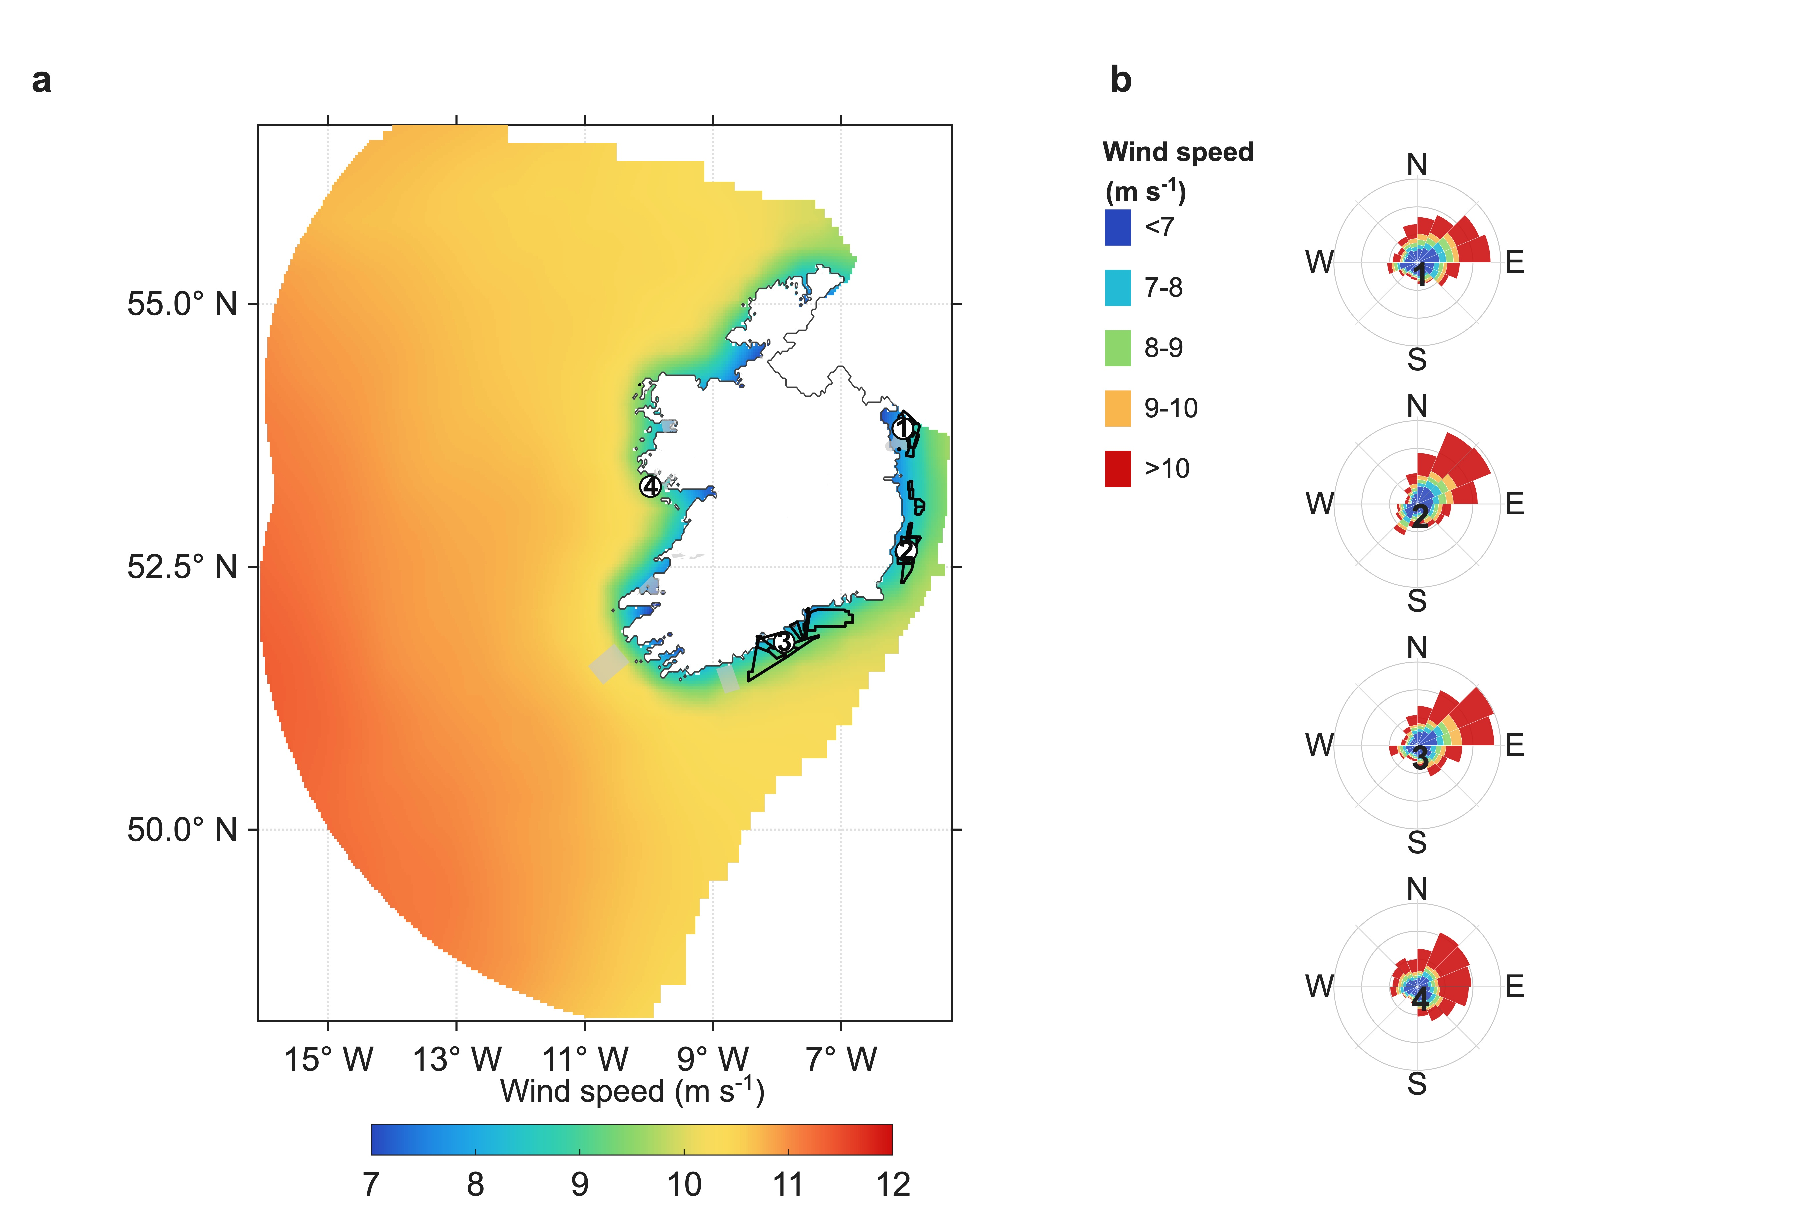
\includegraphics[width = 1\columnwidth]{figs/fig wind speed map.pdf}
    \caption{
    \textbf{Wind velocity distribution in Ireland.} 
    \textbf{a} wind speed distribution, with excluded areas (protected marine sites, military areas, and aquaculture sites) outlined in grey colours;
    \textbf{b} wind roses at current candidate offshore wind areas, with locations marked in \textbf{a}.}
    \label{fig wind speed ireland}
\end{figure}

The ten years of historical weather data, including wind velocity, temperature, air density, etc., in the assessment areas, are collected from the ERA5 product \cite{ERA5}. The temporal resolution is one hour, and the spatial resolution is 0.25$^\circ$ latitude and 0.25$^\circ$ longitude.
Within the grid, the wind speed and other physical values are interpolated based on inverse square rules. 
Then, the mean wind speed, and its probability distribution of offshore locations are shown in Fig. \ref{fig wind speed ireland}. 


\subsection{Wind turbine model}

The Vestas 15MW wind turbine model is used for calculating the electricity generation associated with the wind speed \cite{V23615}. The physical parameters of the wind turbine are shown in the Table. \ref{tab wind turbine para}. Its power curve is shown in Fig. \ref{fig electricity curve}. When the wind speed exceeds the ''cut-in" speed, the wind turbine begins to generate power, which increases gradually to the rated power with the rated wind speed. Then, the electricity generation remains the same, and decreases to zero if the wind exceeds the ''cut-out" speed.

\begin{table}[]
\caption{Physical parameters of Vestas V236-15MW wind turbine}
\label{tab wind turbine para}
\begin{tabular}{p{1cm}p{1cm}p{1.5cm}p{1cm}p{1cm}p{2cm}p{2cm}}
\hline
Rated power & Cut-in speed & Cut-out speed & Rotor radius & Hub height & Surface roughness length & Thrust coefficient \\ \hline
15 MW       & 3 m/s        & 31 m/s       & 118 m        & 150 m      & 0.0002                   & 0.5                \\ \hline
\end{tabular}%
\end{table}

\begin{figure}
    \centering
    
\includegraphics[width = 0.8\columnwidth]{figs/fig power curve of wind turbine.pdf}
    \caption{Power generation curve of Vestas V236-15MW wind turbine}
    \label{fig electricity curve}
\end{figure}

\subsection{Wake effect}

When forming a wind turbine fleet, the wind speed downstream may be interfered with by upstream turbines when the wind passes through the blades. This is known as the wake effect, where such a wind decrease can result in reductions in power generation. 

\begin{figure}
    \centering
    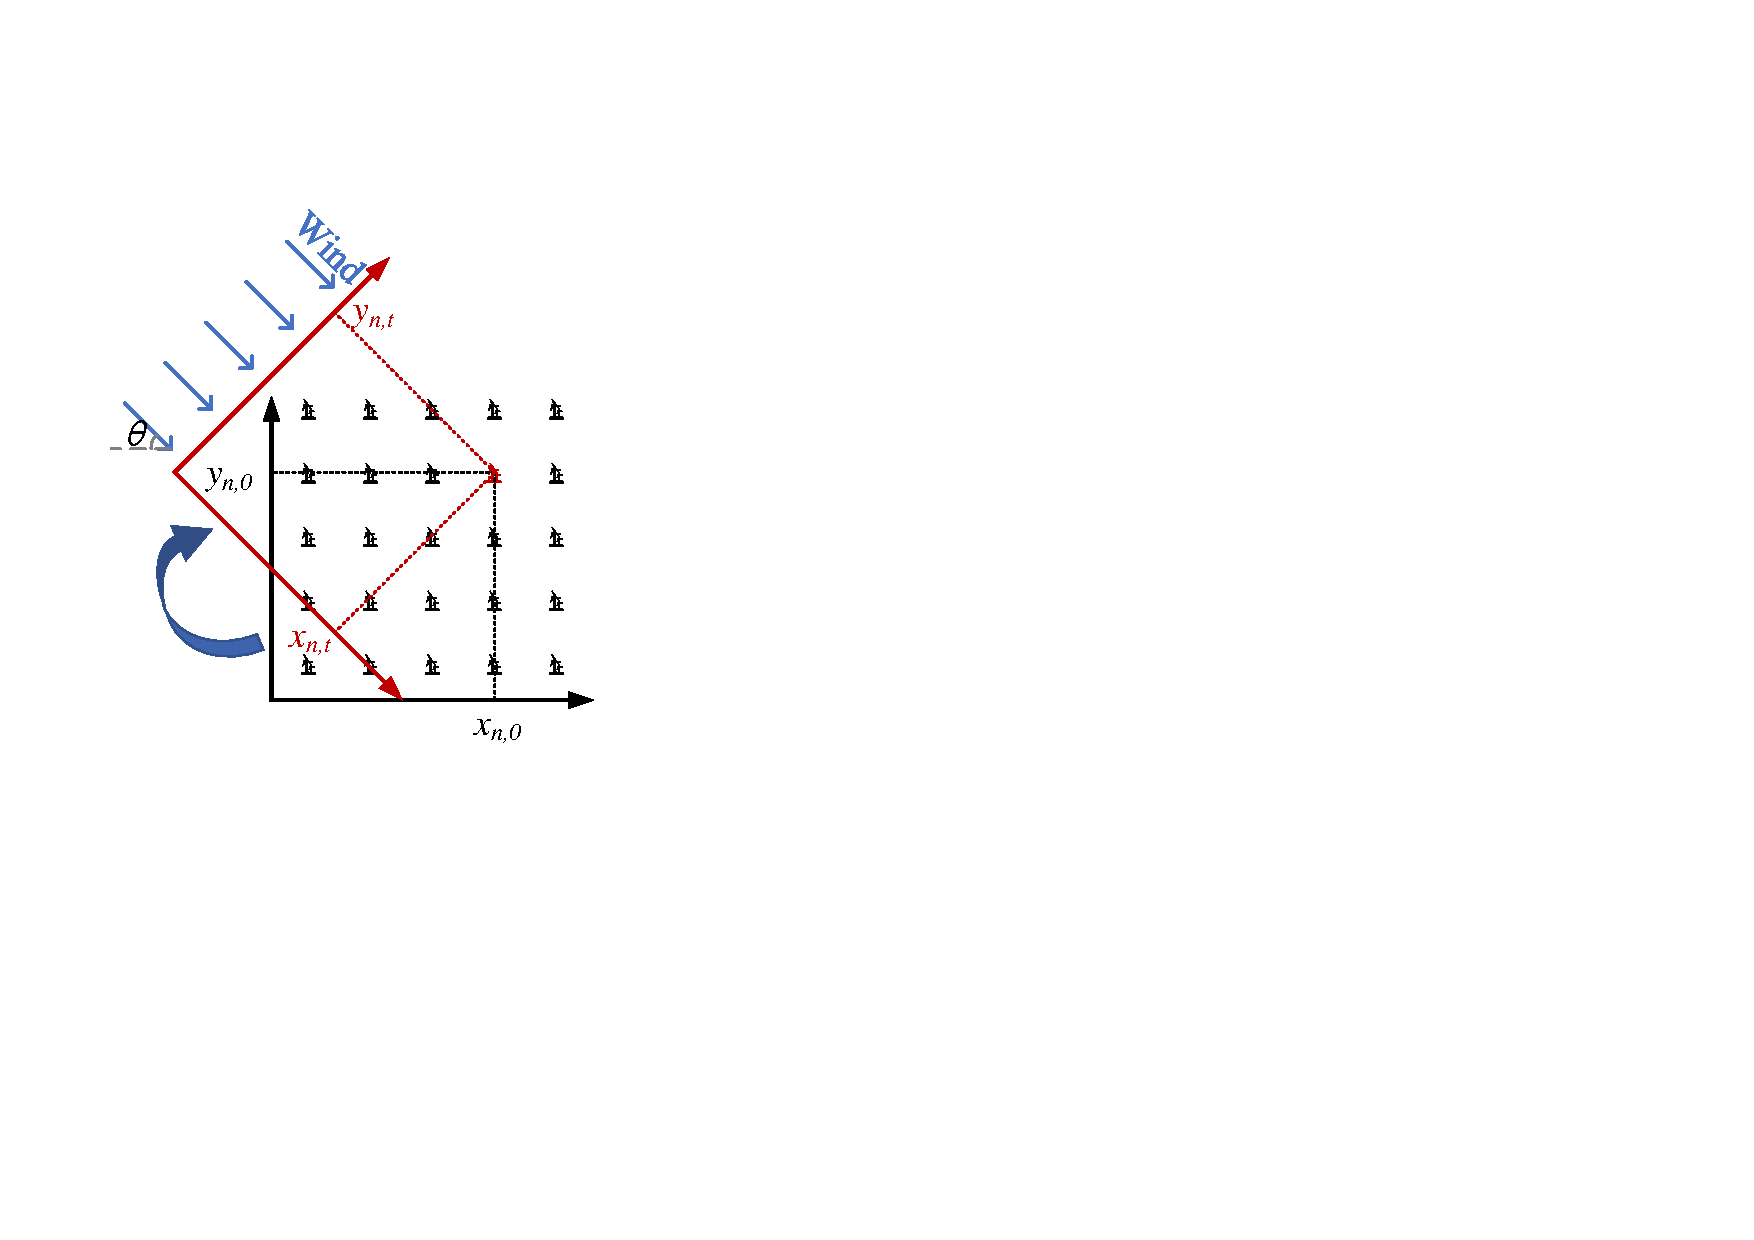
\includegraphics[width = 0.4\columnwidth]{figs/fig coordinate conversion.pdf}
    \caption{Rotation of coordinate axis with the change of wind directions}
    \label{fig coordinate rotation}
\end{figure}

The wind velocity is a vector described by two dimensions, namely, speed $v$ and angle $\theta$ (the angle between the wind direction and the equator. To calculate the wake effect, the coordinate axes need to be built and shifted constantly as the wind angle changes, as shown in Fig.\ref{fig coordinate rotation}. Then, the new coordinates of wind turbine $n$ at time $t$ ($x'_{n,t}$,$y'_{n,t}$) can be converted by:
\begin{gather}
    \begin{bmatrix}
    x_{n,t} \\
    y_{n,t}
    \end{bmatrix}
    = 
    \begin{bmatrix}
    \cos{\theta} & -\sin{\theta} \\
    \sin{\theta} & \cos{\theta}
    \end{bmatrix}
    \begin{bmatrix}
    x_{n,0} \\
    y_{n,0}
    \end{bmatrix}
\end{gather}
where $x_{n,0}$ and $y_{n,0}$ are the original geographical coordinates of WT $n$ (longitude and latitude) before converting.

After rotation, the wind direction is always parallel to the x-axis. Then, we calculate the wake effect using the Jensen-Gaussian wake model. The wind speed decrease factor at an downstream location $(x,y)$ can be calculated as \cite{tao2019optimal}:
\begin{align}
    \delta v_{n_1} = v_{n_1} \left(\left(1-\sqrt{1-\frac{C^T}{2 (\omega / R_{n_1} )^2}}\right) e^{-\frac{\Delta y^2}{2\omega^2}}\right)
\end{align}
where $v_{n_1}$ is the wind speed at the location of WT $n_1$; $C^T$ is the WT thrust coefficient; $R_{n_1}$ is the rotor radius; $\Delta y = |y-y_{n_1}|$ is the distance in latitude; $\omega$ is the characteristic width of the wake, which is calculated by \cite{tao2019optimal}:
\begin{gather}
    \omega = \left(R_{n_1} + 0.56 / (\ln{z^h} - \ln{z_0}) \Delta x \right)/2
\end{gather}
where $z^h$ is the WT hub height, and $z_0$ is the surface roughness length; $\Delta x = x-x_{n_1}, x \geq x_{n_1}$ is the difference in longitude. 

The simulation results of Vestas V236-15MW wind turbine are presented in Fig. \ref{fig wake effect simulation}. As can be observed from both the figure and formulations, we notice that the wake effect decreases with the increase of $x$ and $y$. When the wind is at a certain range of angles, the upstream wind turbine could significantly affect the operation of downstream ones. To minimise the interference, we outline the red line, as in Fig. \ref{fig wake effect simulation},  the areas where the wind speed decreases by the wake effect would exceed 5\%. Yearly historical wind data is used for determining the minimum distance between wind turbines, which requires the interference from adjacent wind turbines to be less than 5\%. This distance is $d^{min} = 2.31 km$.

\begin{figure}
    \centering
    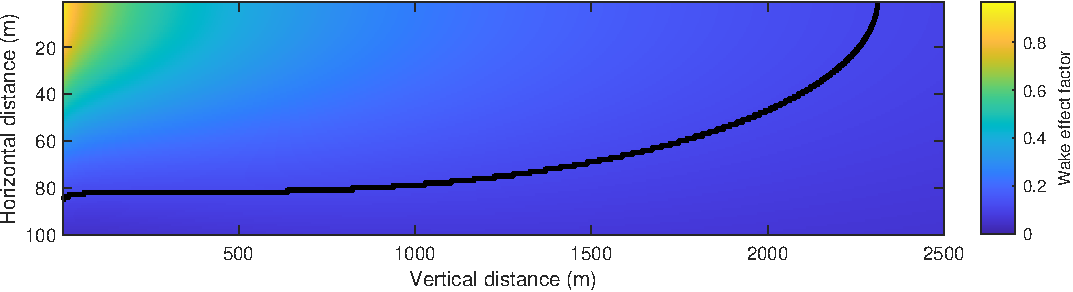
\includegraphics[width = 1\columnwidth]{figs/fig wake effect single.pdf}
    \caption{Simulation of the wake effect of a single wind turbine. The black line separates the areas with an annual wake effect of less than 5\% and areas higher than 5\%.}
    \label{fig wake effect simulation}
\end{figure}

\section{Offshore hydrogen and other chemical products cost models}
\label{sec cost}

\subsection{Summary of several technical routes}
Several technical routes are considered in utilising the offshore wind, as shown in Fig. \ref{fig technical routes}, including:

\begin{figure}
    \centering
    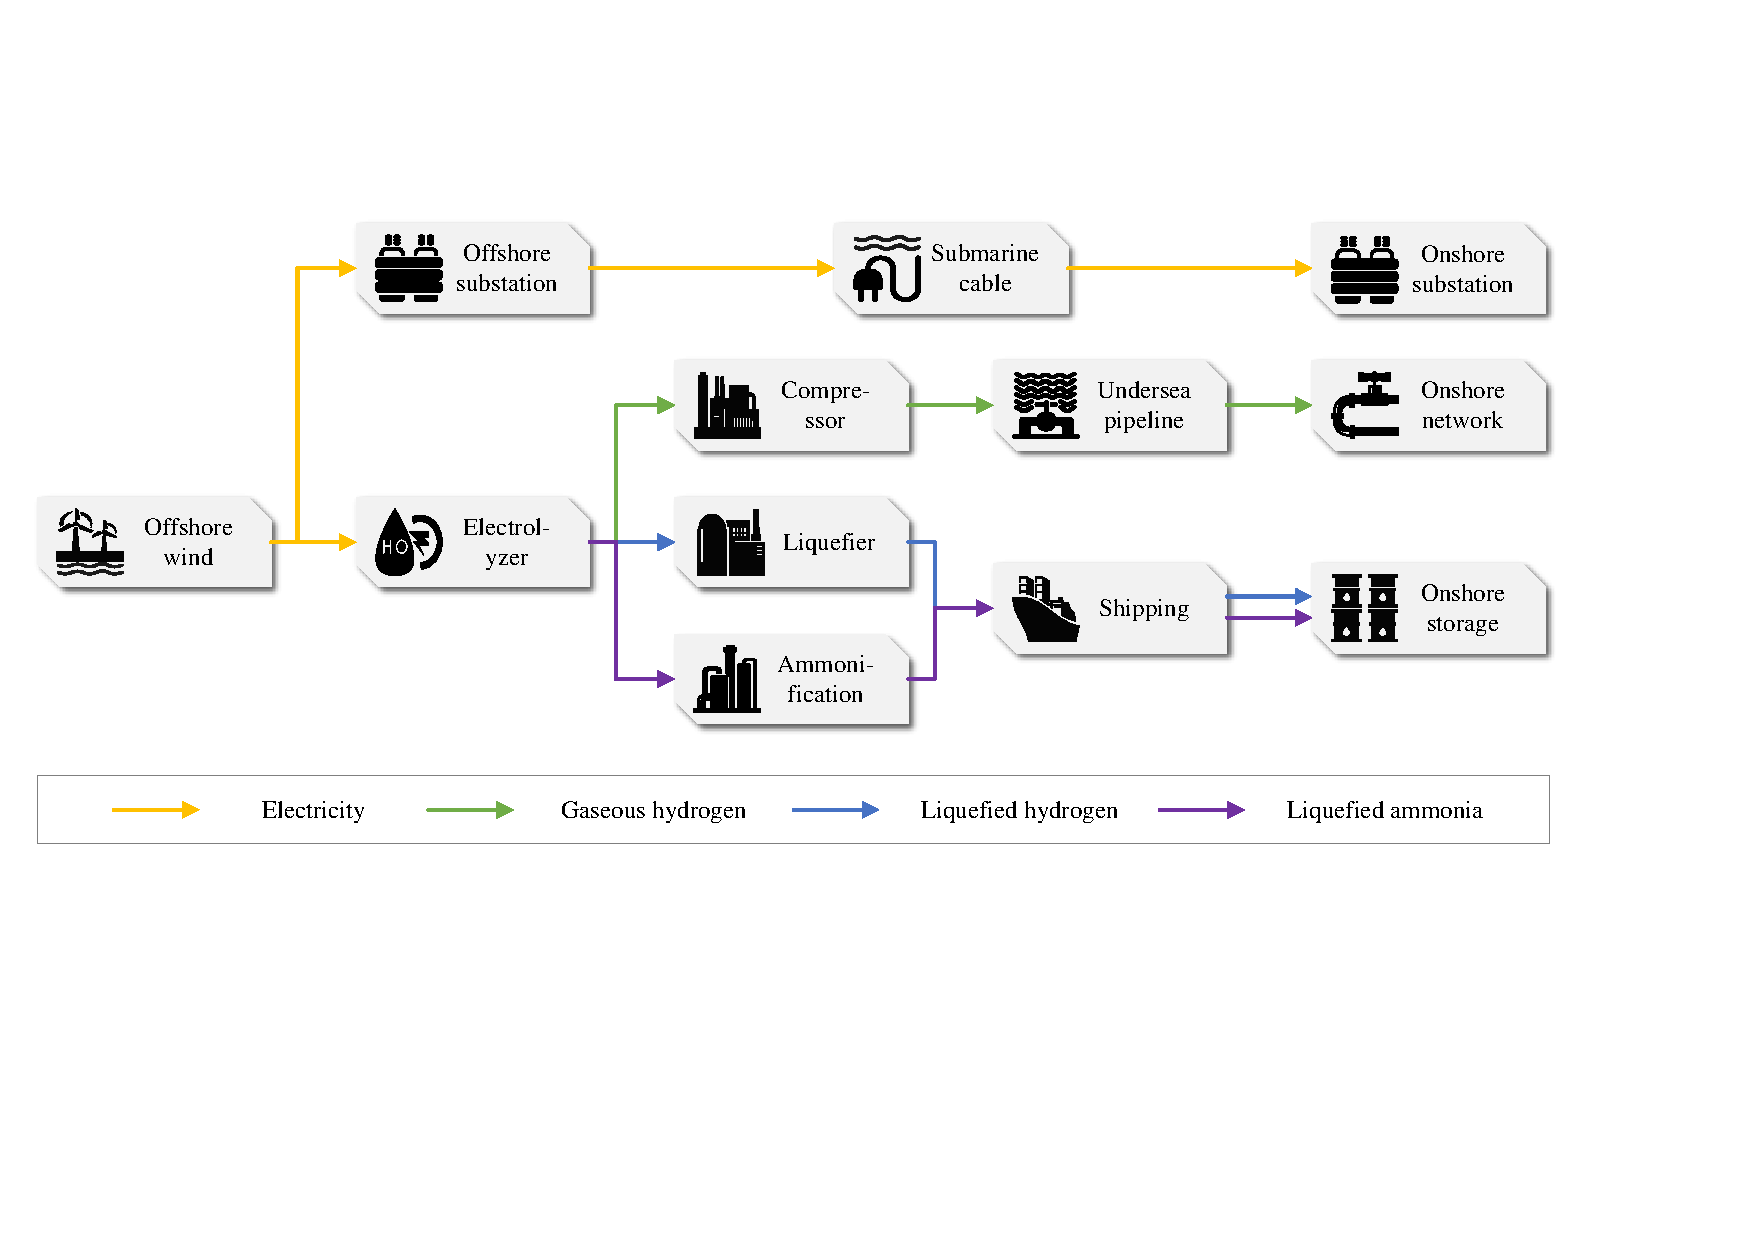
\includegraphics[width = 0.99\columnwidth]{figs/fig technical route.pdf}
    \caption{Technical Routes for using offshore resources}
    \label{fig technical routes}
\end{figure}

\begin{enumerate}
    \item Electricity: The electricity generated from offshore wind will be collected at an offshore substation, and through submarine cables, it will be connected to onshore substations. Given the lower investment cost, the electricity transmission cost will have a lower levelised cost of electricity (LCOE). However, due to the limitation of the length of the submarine cables, the offshore wind electricity will only be transported to the nearest onshore power system, so the transmission distance will be limited. Moreover, the transmission capacity not only depends on the investment in submarine cables, but also relies on the capacity of the onshore connection points, which is further related to the structure and operating strategies of the onshore power systems. Therefore, this issue needs to be further discussed in the next section.
    \item Compressed gaseous hydrogen: The green hydrogen produced from electrolysers can be compressed and transported to the onshore gas system. Considering the large volume of hydrogen, network transmission will be more cost-effective. The hydrogen injection into the gas network, also known as hydrogen blending, has an upper limit for hydrogen molar fraction, which will affect the integration capability of hydrogen. Details will be discussed in the next section. Moreover, similar to electricity transmission solutions, undersea pipelines also have length limitations, which means the offshore hydrogen can only be transported to nearby countries. 
    \item Liquefied hydrogen: After hydrogen is further liquefied, it has a higher energy density, and can be shipped internationally.
    \item Liquefied ammonia: The hydrogen can be further converted to ammonia through Haber-Bosch Reactors. Compared with liquefied hydrogen, the energy density is higher and thus is more suitable for long-distance and time-sensitive transportation. However, if the destination can not directly use or burn ammonia and has to convert it back to hydrogen, then it will generate additional cost and energy loss.
\end{enumerate}

\subsection{Route 1: electricity transmission}

The evaluation structure of LCOE of offshore wind electricity is presented in Fig. \ref{fig LCOE composition}. The total life cycle cost is divided into development expenditure (DEVEX), capital expenditure (CAPEX), operating expenditure (OPEX), and decommissioning expenditure (DECEX). They are converted into net present value to calculate the LCOE:
\begin{gather}
    LCOE = \frac{DEVEX + CAPEX + \sum_{t=1}^{t=T} OPEX_t (1+r)^{-(t-1)} + DECEX^{T-1}}
   {8760 P^{owf,rated} \times CF \times LF \times T}
\label{eq LCOE calculation}
\end{gather}
where $t$ is the index for year; $T$ is the total year of lifetime; $OPEX_t$ represents the OPEX in year $t$; $r$ is the discount rate; $P^{owf,rated}$ is the rated power of the offshore wind farm (OWF); $CF$ and $LF$ are the capacity factor and load factor of the OWF, respectively, which is calculated based on yearly simulation and historical wind data.
In the following content, each component is introduced in detail.

\begin{figure}
    \centering
    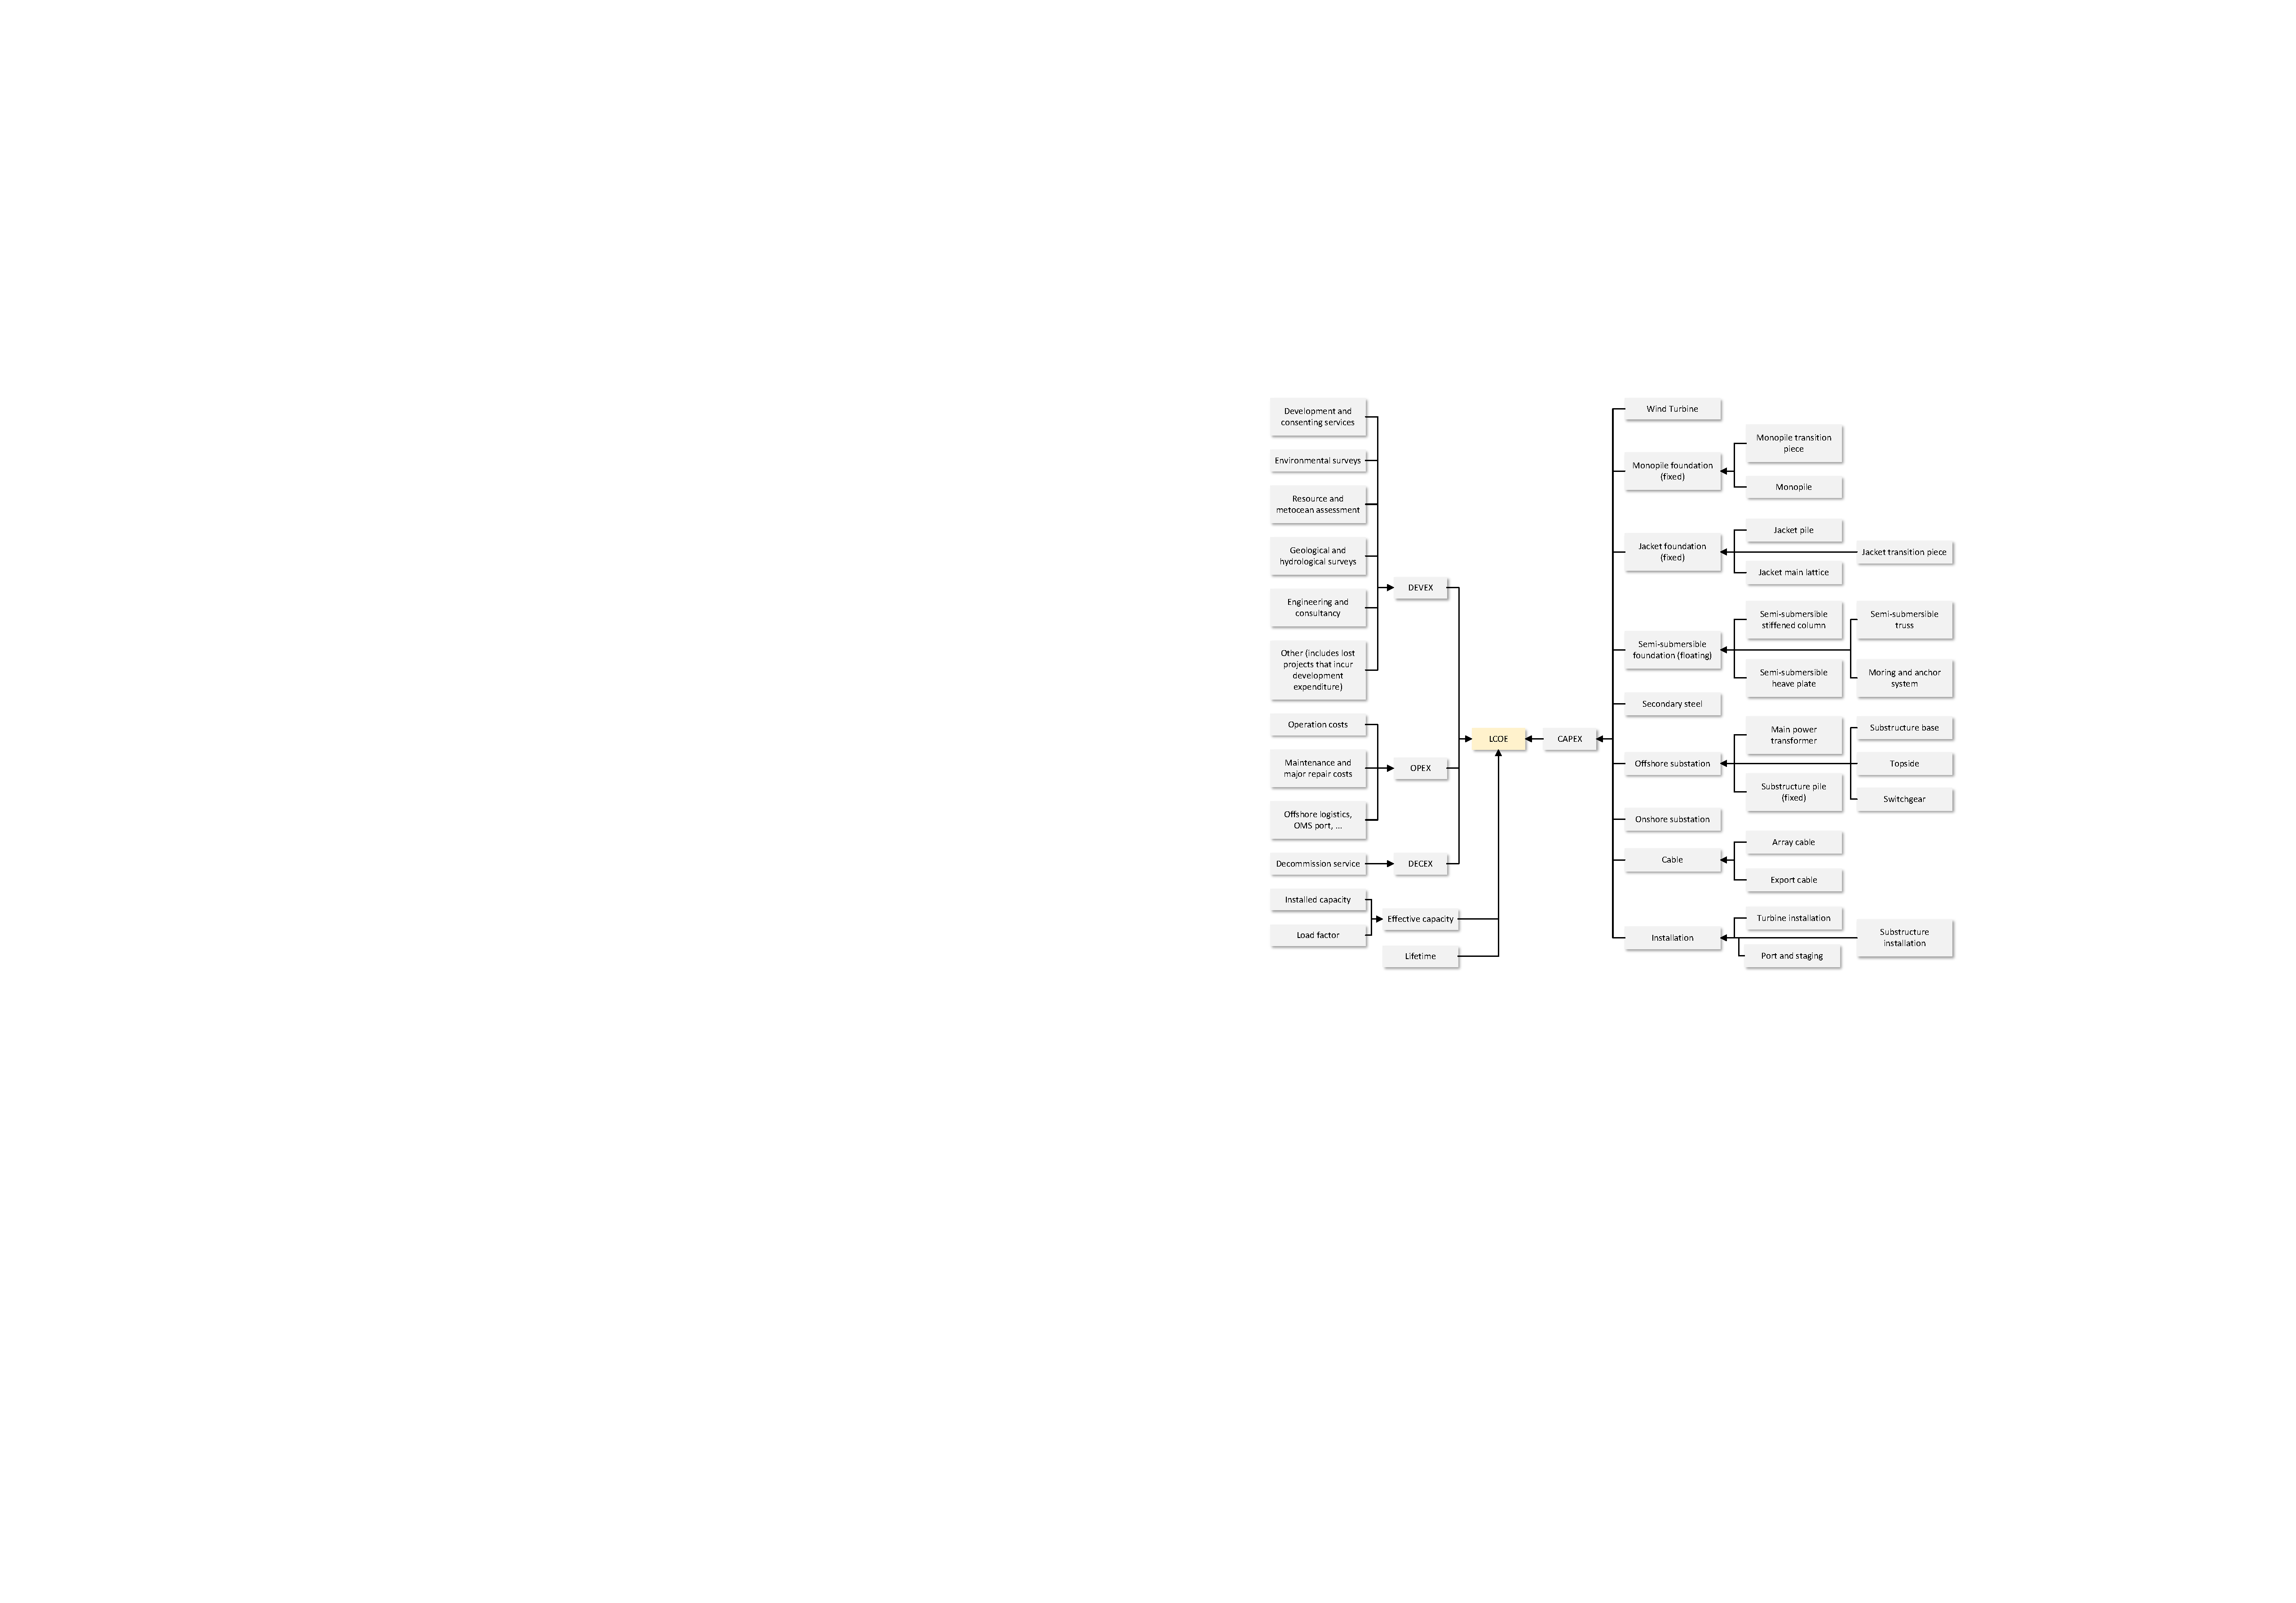
\includegraphics[width = 0.99\columnwidth]{figs/fig LCOE structure.pdf}
    \caption{Calculation of LCOE}
    \label{fig LCOE composition}
\end{figure}

(1) DEVEX

DEVEX includes development and consenting services, environmental surveys, resource and metocean assessment, geological and hydrological surveys, engineering and consultancy, and other development costs. The data are derived from a typical reference value from a UK OWF project, as shown in the Table.\ref{tab devex cost} \cite{Guidetoanoffshorewindfarm}.

\begin{table}
    \centering
    \caption{DEVEX cost items \cite{Guidetoanoffshorewindfarm}}
    \begin{tabular}{cc}
    \hline
        Items in DEVEX & Cost (\pounds /MW)\\
    \hline
         Development and project management & 5000 \\
         Environmental survey & 4000 \\
         Resource and metocean assessment & 4000\\
         Geological and hydrological surveys & 4000\\
         Engineering and consultancy & 4000\\
         Other costs & 54000 \\
     \hline
    \end{tabular}
    \label{tab devex cost}
\end{table}

(2) CAPEX

(2.1) Wind turbine

Generally, we assume the capital cost of wind turbines holds a linear relationship to the capacity. According to linear regression based on the available dataset of offshore wind projects, this relationship can be expressed as (for large capacity wind turbines) \cite{dinh2023geospatial, maienza2020life}:
\begin{gather}
    C^{wt} =  (1.6 P^{wt,rated} - 1.9) \times 10^6
\end{gather}
where $C^{wt}$ is the capital cost of wind turbine, and $P^{wt,rated}$ is its rated power.

(2.2) Mono-pile foundation

Three foundations are considered, including mono-pile, jacket, and semi-submersible platforms. The first two are used for fixed offshore wind. The mono-pile foundation is usually used in sandy and gravelly compositions, with water depths of 0-30m. and the jacket is preferred to be used on the non-rocky ground, with water depth from 30-60m. Semi-submersible platforms are used for floating offshore wind in faraway areas. As shown in Fig. \ref{fig water depth}, the black and red lines separate the mono-pile, jacket, and semi-submersible areas in European marine areas \cite{bathymetry2022}. It can be seen that usually the fixed platform can only be deployed in coastal areas, but in the southeast part of the North Sea (near Denmark and Germany), the marine areas suitable for fixed-bottom offshore wind platforms can extend a considerable distance from the land.

\begin{figure}
    \centering
    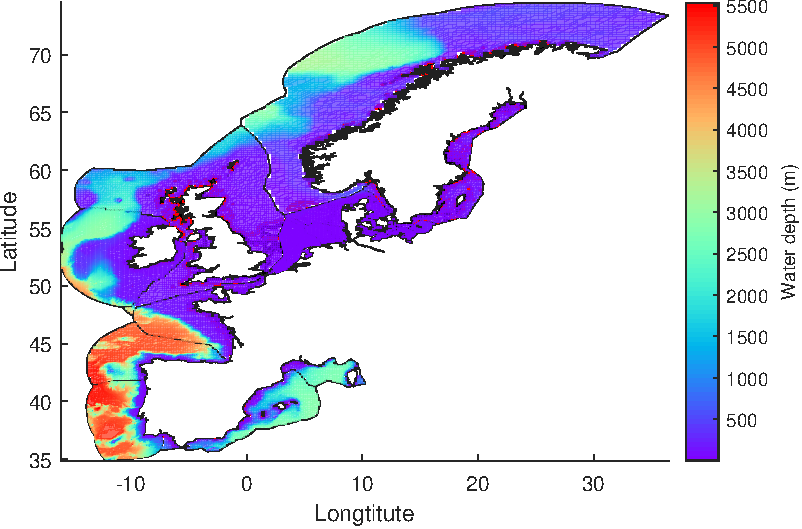
\includegraphics[width = 0.99\columnwidth]{figs/fig water depth map.pdf}
    \caption{Exclusive Economic Zone, water depth, and offshore foundation separation of coastal European countries. The black and red lines separate the marine areas that are more suitable for mono-pile, jacket, and semi-submersible platforms, respectively. Major coastal countries are analysed in this paper (including Belgium (BE), Denmark (DK), France (FR), Germany (DE), Ireland (IE), Netherlands (NL), Norway (NO), Portugal (PT), Spain (ES), Sweden (SE), and the UK (GB)). }
    \label{fig water depth}
\end{figure}

Mono-pile foundation includes the mono-pile structure and transition piece, where the capital cost is calculated based on the mass used in the structure. The mass is fitted based on data in recently committed offshore wind projects \cite{NRELOffshoreBalance}:
\begin{gather}
    M^{mono-pile} = 10^{-4} \bigg( (10^3 P^{wt,rated})^{1.5} + 10^{-1}(H^{wt})^{3.7} 
\notag \\
    + 2100(H^{wd})^{2.25} + (10^3 M^{rna})^{1.13} \bigg)
\\
    M^{mono-trans} = e^{3.712.77 + 1.04(P^{wt,rated})^{0.5} + 0.00127(H^{wd})^{1.5}}
\end{gather}
where $M^{mono-pile}$ and $M^{mono-trans}$ are the masses of mono-pile and transition piece, respectively; $P^{wt,rated}$ is the rated power of the wind turbine; $H^{wd}$ is the water depth; $M^{rna}$ is the rotor nacelle assembly mass, which can be calculated as:
\begin{gather}
    M^{rna} = 2.082 (P^{wt,rated})^2 + 44.59 P^{wt,rated} + 22.48
\end{gather}

Then, the capital cost of the mono-pile foundation can be calculated by:
\begin{gather}
    C^{mono} = \rho^{mono-pile} M^{mono-pile} + \rho^{mono-trans} M^{mono-trans}
\end{gather}
where $\rho^{mono-pile}$ and $\rho^{mono-transition}$ are the cost rates of mono-pile and transition piece materials. The cost rates (€/ton) of the materials are fitting according to the offshore wind project cost data points in the UK \cite{Guidetoanoffshorewindfarm}:

(2.3) Jacket foundation

The mass of the jacket foundation (including the main lattice, transition piece, and pile), $M^{jacket-ml}$, $M^{jacket-tp}$, and $M^{jacket-pile}$, can be calculated as \cite{NRELOffshoreBalance}:
\begin{gather}
    M^{jacket-ml} = e^{3.71 + 0.00176(P^{wt,rated})^{2.5} + 0.645\ln \left( {(H^{wd})}^{1.5}\right)}
\\
    M^{jacket-tp} = 
    \left( \frac{-0.0131+0.0381}{\ln{P^{wt,rated}}} -2.27\times 10^{-9} (H^{wd})^3 \right)^{-1} 
\\
    M^{jacket-pile} = 8 e^{0.5574 \left(3.71 + 0.00176(P^{wt,rated})^{2.5} + 0.645\ln \left( {(H^{wd})}^{1.5}\right)\right)}
\end{gather}

Then, the total cost of the jacket foundation can be calculated as:
\begin{align}
    C^{jacket} = & \rho^{jacket-ml} M^{jacket-ml} + \rho^{jacket-tp} M^{jacket-tp} 
    \notag\\
    & + \rho^{jacket-pile} M^{jacket-pile}
\end{align}
where $\rho^{jacket-ml}$, $\rho^{jacket-tp}$, and $\rho^{jacket-pile}$ are the cost rates of the main lattice, transition piece, and pile of jacket foundation, respectively.

(2.4) Semi-submersible foundation

The semi-submersible foundation includes a stiffened column, truss, heave plate, and mooring and anchor system. Their mass are denoted as $M^{semi-sc}$, $M^{semi-tr}$, and $ M^{semi-hp}$ can be calculated as \cite{NRELOffshoreBalance,gonzalez2024techno}:
\begin{align}
    M^{semi-sc} = -0.9571(P^{wt,rated})^2 + 40.89(P^{wt,rated}) + 802.09
\\
    M^{semi-tr} = 2.7894 (P^{wt,rated})^2 + 15.591 P^{wt,rated} + 266.03
\\
    M^{semi-hp} = - 0.4397 (P^{wt,rated})^2 + 21.545 P^{wt,rated} + 177.42
\end{align}

Additionally, the cost of mooring and anchor system $C^{mo}$ can be calculated as:
\begin{align}
    C^{mo} = N^{wt} N^{lin} (C^{anc} + (1.5 H^{wd} + 410) C^{lin} + 50 C^{ch})
\end{align}
where $N^{wt}$ is the number of wind turbines; $N^{lin}$ is the number of mooring lines per turbine or floater (assumed to be 4 in this study); $C^{anc}$ is the cost of an individual anchor; $C^{lin}$ and $C^{ch}$ are the cost of each mooring line and chain sector per unit of length, respectively.

Then, the costs of semi-submersible $C^{semi}$ can be calculated as:
\begin{gather}
    C^{semi} = \rho^{semi-sc} M^{semi-sc} + \rho^{semi-tr} M^{semi-tr} + \rho^{semi-hp} M^{semi-hp} + C^{mo}
\end{gather}
where $\rho^{semi-sc}$, $\rho^{semi-tr}$, and $\rho^{semi-hp}$ are the cost rates of semi-submersible Stiffened Column, truss, and heave plate, respectively.

(2.5) Secondary steels

Secondary steel refers to the steel used to support the ladders, railings, walkways, etc. The mass of these materials depends on different foundation structures. For a fixed structure, the mass $M^{scd-fx}$ can be calculated as in (\ref{eq secondary steel fixed}); for a semi-submersible foundation, it can be calculated as in (\ref{eq secondary steel semisubmersible}) \cite{NRELOffshoreBalance}:
\begin{gather}
    M^{scd-fx} = 40 + \left(0.8\left(18+H^{wd}\right)\right)
\label{eq secondary steel fixed} \\
    M^{scd-semi} = -0.153(P^{wt,rated})^2 + 6.54 P^{wt,rated} + 128.34
\label{eq secondary steel semisubmersible}
\end{gather}

(2.6) Offshore substation

The offshore substation mainly consists of electrical facilities (main power transformers, switchgear for HVDC transportation) and supporting structures (topside structures, foundation platforms and bottom piles). 

The main power transformers' total capacity must match the OWF's capacity. Usually, we set 0.2 times redundancy \cite{guo2023grid}. Then, the number of main power transformers can be calculated as:
\begin{align}
    N^{mpt} = \lceil{1.2 P^{owf,rated} /  P^{mpt,rated}}\rceil
\end{align}
where $P^{mpt,rated}$ = 300 MVA is the capacity of the main power transformer. 

The switchgear isolates and protects the key electrical equipment and helps with the conversion of voltage. It contains high-voltage and mid-voltage ones, whose number matches the number of the main power transformer, i.e., $N^{switchgear} = N^{mpt}$.

The topside structure of the substation contains the spaces in the offshore substation. The mass of topside structure $M^{offsub-top}$ is also fitted from the project data, with respect to the properties of main power transformers \cite{NRELOffshoreBalance}:
\begin{align}
    M^{offsub-top} = 3.85 (P^{mpt,id} N^{mpt}) + 285
\end{align}

Other substation foundation structures depend on the type of OWF. For fixed structure, the mass of substation foundation $M^{offsub-fdt-fx}$ can be calculated as:
\begin{gather}
    M^{offsub-fdt-fx} = 40 + (0.8(18+H^{wd}))
\end{gather}

For floating one, the mass $M^{offsub-fdt-fl}$ can be calculated as:
\begin{gather}
    M^{offsub-fdt-fl} = 2(M^{semi} + M^{scd-semi})
\end{gather}

Specifically for fixed foundations, the mass of the supporting pile can be calculated as:
\begin{gather}
    M^{offsub-pile} = 8 (M^{offsub-fdt-fx})^{0.5574}
\end{gather}

Then, the capital cost of the offshore substation can be added up as follows. 
For fixed structure, the cost $C^{offsub-fx}$ can be calculated as:
\begin{gather}
    C^{offsub-fx} = \rho^{mpt} P^{mpt,rated} N^{mpt} + (\rho^{switch-hv} 
\notag\\
    + \rho^{switch-mv}) N^{switch} + \rho^{offsub-top} M^{offsub-top} 
    \notag\\
    + \rho^{offsub-fdt-fx} M^{offsub-fd-fx} + \rho^{offsub-pile} M^{offsub-pile}
\end{gather}
where $\rho^{mpt}$, $\rho^{switch-hv}$, $\rho^{switch-mv}$, $\rho^{offsub-top}$, and $\rho^{offsub-fdt-fx}$ are the unit costs of main power transformer, high-voltage and medium-voltage switchgear, topside materials, and fixed foundation, respectively.

For floating structure, the cost $C^{offsub-fl}$ can be calculated as:
\begin{gather}
    C^{offsub-fl} = \rho^{mpt} P^{mpt,rated} N^{mpt} + (\rho^{switch-hv} 
\notag\\
    + \rho^{switch-mv}) N^{switch} + \rho^{offsub-top} M^{offsub-top} 
\notag\\
    + \rho^{offsub-fdt-fl} M^{offsub-fdt-fl}
\end{gather}
where $\rho^{offsub-fdt-fl}$ is the unit cost of the floating foundation.

(2.7) Onshore substation

The onshore substation cost $C^{onsub}$ can be calculated as:
\begin{gather}
    C^{onsub} = 11652(V_i+P^{owf,rated}) + 1.2 \times 10^6
\end{gather}
where $V_i$ is the voltage level at the interconnection point of the offshore wind.

(2.8) Submarine cables

The submarine cables can be divided into export cables and array cables, where array cables merge the power generation of the wind turbine to the offshore substation, and export cables transport the electricity to the onshore substation.
The number of DC array cables $N^{cb-ar}$ are calculated based on the rated powers of the cables and wind turbines, and some marginal power is reserved for redundancy \cite{guo2023grid}. Here, we assume the shortest path of the array cable connection, and then the number of links between wind turbines is approximately equal to the number of wind turbines. Then, we have:
\begin{gather}
    N^{cb-ar} = N^{wt} \lceil 1.1 P^{wt,rated} / P^{cb-ar,rated} \rceil
\end{gather}
where $P^{cb-ar,rated}$ is the rated power of the candidate array cables.

The cost of the array cable depends on the length of each array cable, which is further related to the structure of the wind turbines. For fixed foundation:
\begin{gather}
    C^{cb-ar-fx} = 0.1 \sqrt{P^{cb-ar,rated}} N^{cb-ar} \times 1.1 (D^{wt}+2H^{wd}) 
\end{gather}
where $D^{wt}$ is the distance between wind turbines, which is determined based on the minimum wind turbine distance that could minimise the wake effect calculated in Section \ref{sec offshore wind farm model}.

For floating structures:
\begin{gather}
    C^{cb-ar-fl} = 0.1 \sqrt{P^{cb,rated}} N^{cb-ar} \times 1.1 (2H^{wd}/\cos{(\theta^{hg})} + D^{wt})
\end{gather}
where $\theta^{hg}$ is the hanging angle, which can be calculated by \cite{NRELOffshoreBalance}:
\begin{gather}
    \theta^{hg} = -0.0047H^{wd}+18.743)/180\times \pi)
\end{gather}

Similarly, the number of export cables is calculated based on the total capacity of the OWF:
\begin{gather}
    N^{cb-ex} = \lceil 1.1 P^{owf,rated} / P^{cb-ex,rated} \rceil
\end{gather}

Then, the costs of export cable for fixed and floating structures can be calculated as (\ref{eq cost export cable fixed}) and (\ref{eq cost export cable floating}), respectively:
\begin{gather}
    C^{cb-ex-fx} =  0.1 \sqrt{P^{cb-ex,rated}} N^{cb-ex} \times 1.1 (2 H^{wd} + D^{cn})
\label{eq cost export cable fixed} \\
    C^{cb-ex-fl} =  0.1 \sqrt{P^{cb-ex,rated}} N^{cb-ex} \times 1.1 (2 H^{wd}/\cos{(\theta^{hg})} + D^{cn})
\label{eq cost export cable floating} 
\end{gather}
where $D^{cn}$ is the distance between the OWF and the nearest connection point, which can be calculated as:
\begin{gather}
    D^{cn} = \min_{i \in \mathcal{I}^{E}} ||x^{owf}-x_i, y^{owf}-y_i||_2
\label{eq distance to power bus}
\end{gather}
where $i$ is the index for the electric bus; $\mathcal{I}^{E}$ is the set of all the electric buses; coordinate $x_i$ and $y_i$ represent the longitude and latitude of electric bus $i$, and $x^{owf}$ and $y^{owf}$ are the longitude and latitude of the OWF, respectively.

(2.9) Installation cost

The installation cost consists of three parts: substructure installation cost, turbine installation cost, and port/staging cost. They are fitted based on recently committed OWF project data, which can be found in \cite{ASpatialEconomic}.
Summarising all capital cost items and the installation cost, the CAPEX can be calculated depending on the structure of the OWF. The mono-pile, jacket, and semi-submersible types of offshore wind are calculated in (\ref{eq capex mono}), (\ref{eq capex jacket}), and (\ref{eq capex jacket}), respectively.
\begin{gather}
    CAPEX = N^{wt} \left( C^{wt} + C^{mono} + C^{scd-fx} + C^{cb-ar-fx} \right) + C^{offsub-fx} \notag\\
    + C^{onsub} + C^{cb-ex-fx} + C^{int}
\label{eq capex mono} \\
    CAPEX = N^{wt} \left( C^{wt} + C^{jacket} + C^{scd-fx} + C^{cb-ar-fx} \right) + C^{offsub-fx} 
    \notag\\
    + C^{onsub} + C^{cb-ex-fx} + C^{int}
\label{eq capex jacket} \\
    CAPEX = N^{wt} \left( C^{wt} + C^{semi} + C^{scd-fl} + C^{cb-ar-fl} \right) + C^{offsub-fl} 
    \notag\\
    + C^{onsub} + C^{cb-ex-fl} + C^{int}
\label{eq capex semi}
\end{gather}
where $C^{int}$ is the installation cost.

(3) OPEX

The OPEX includes the operation and maintenance costs. The yearly cost is mainly related to the distance of the OWF to the nearest port. This relationship is also derived based on committed project data \cite{ASpatialEconomic}. For fixed OWF, we have (\ref{eq opex fixed}); for floating one, we have (\ref{eq opex floating}).
\begin{gather}
    OPEX_t = (2.5522 \ln(D^{port}) + 90.899) \times 10^6
\label{eq opex fixed}\\
    OPEX_t = (4.0739 \ln(D^{port}) + 76.993) \times 10^6
\label{eq opex floating}
\end{gather}
where the locations of major ports in Europe can be found in \cite{EMODnet}, as presented in Fig. \ref{fig distance to port}.


\begin{figure}
    \centering
    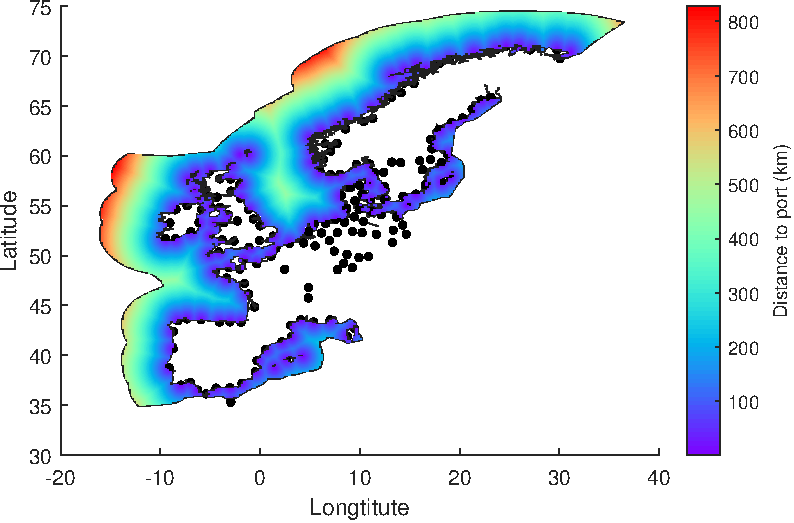
\includegraphics[width = 0.99\columnwidth]{figs/fig distance to port.pdf}
    \caption{Distance to major ports. Black dots represent the location of ports}
    \label{fig distance to port}
\end{figure}

(4) DECEX

The DECEX is assumed to be proportional to the installation cost. The value of the proportion $\alpha$ is derived from recent UK projects \cite{Guidetoanoffshorewindfarm}. It can be calculated as:
\begin{gather}
    DECEX = \alpha^{decex} C^{int}
\end{gather}
where $\alpha^{decex}$ are the decommissioning factor.

\subsection{Route 2: hydrogen production}

\begin{figure}
    \centering
    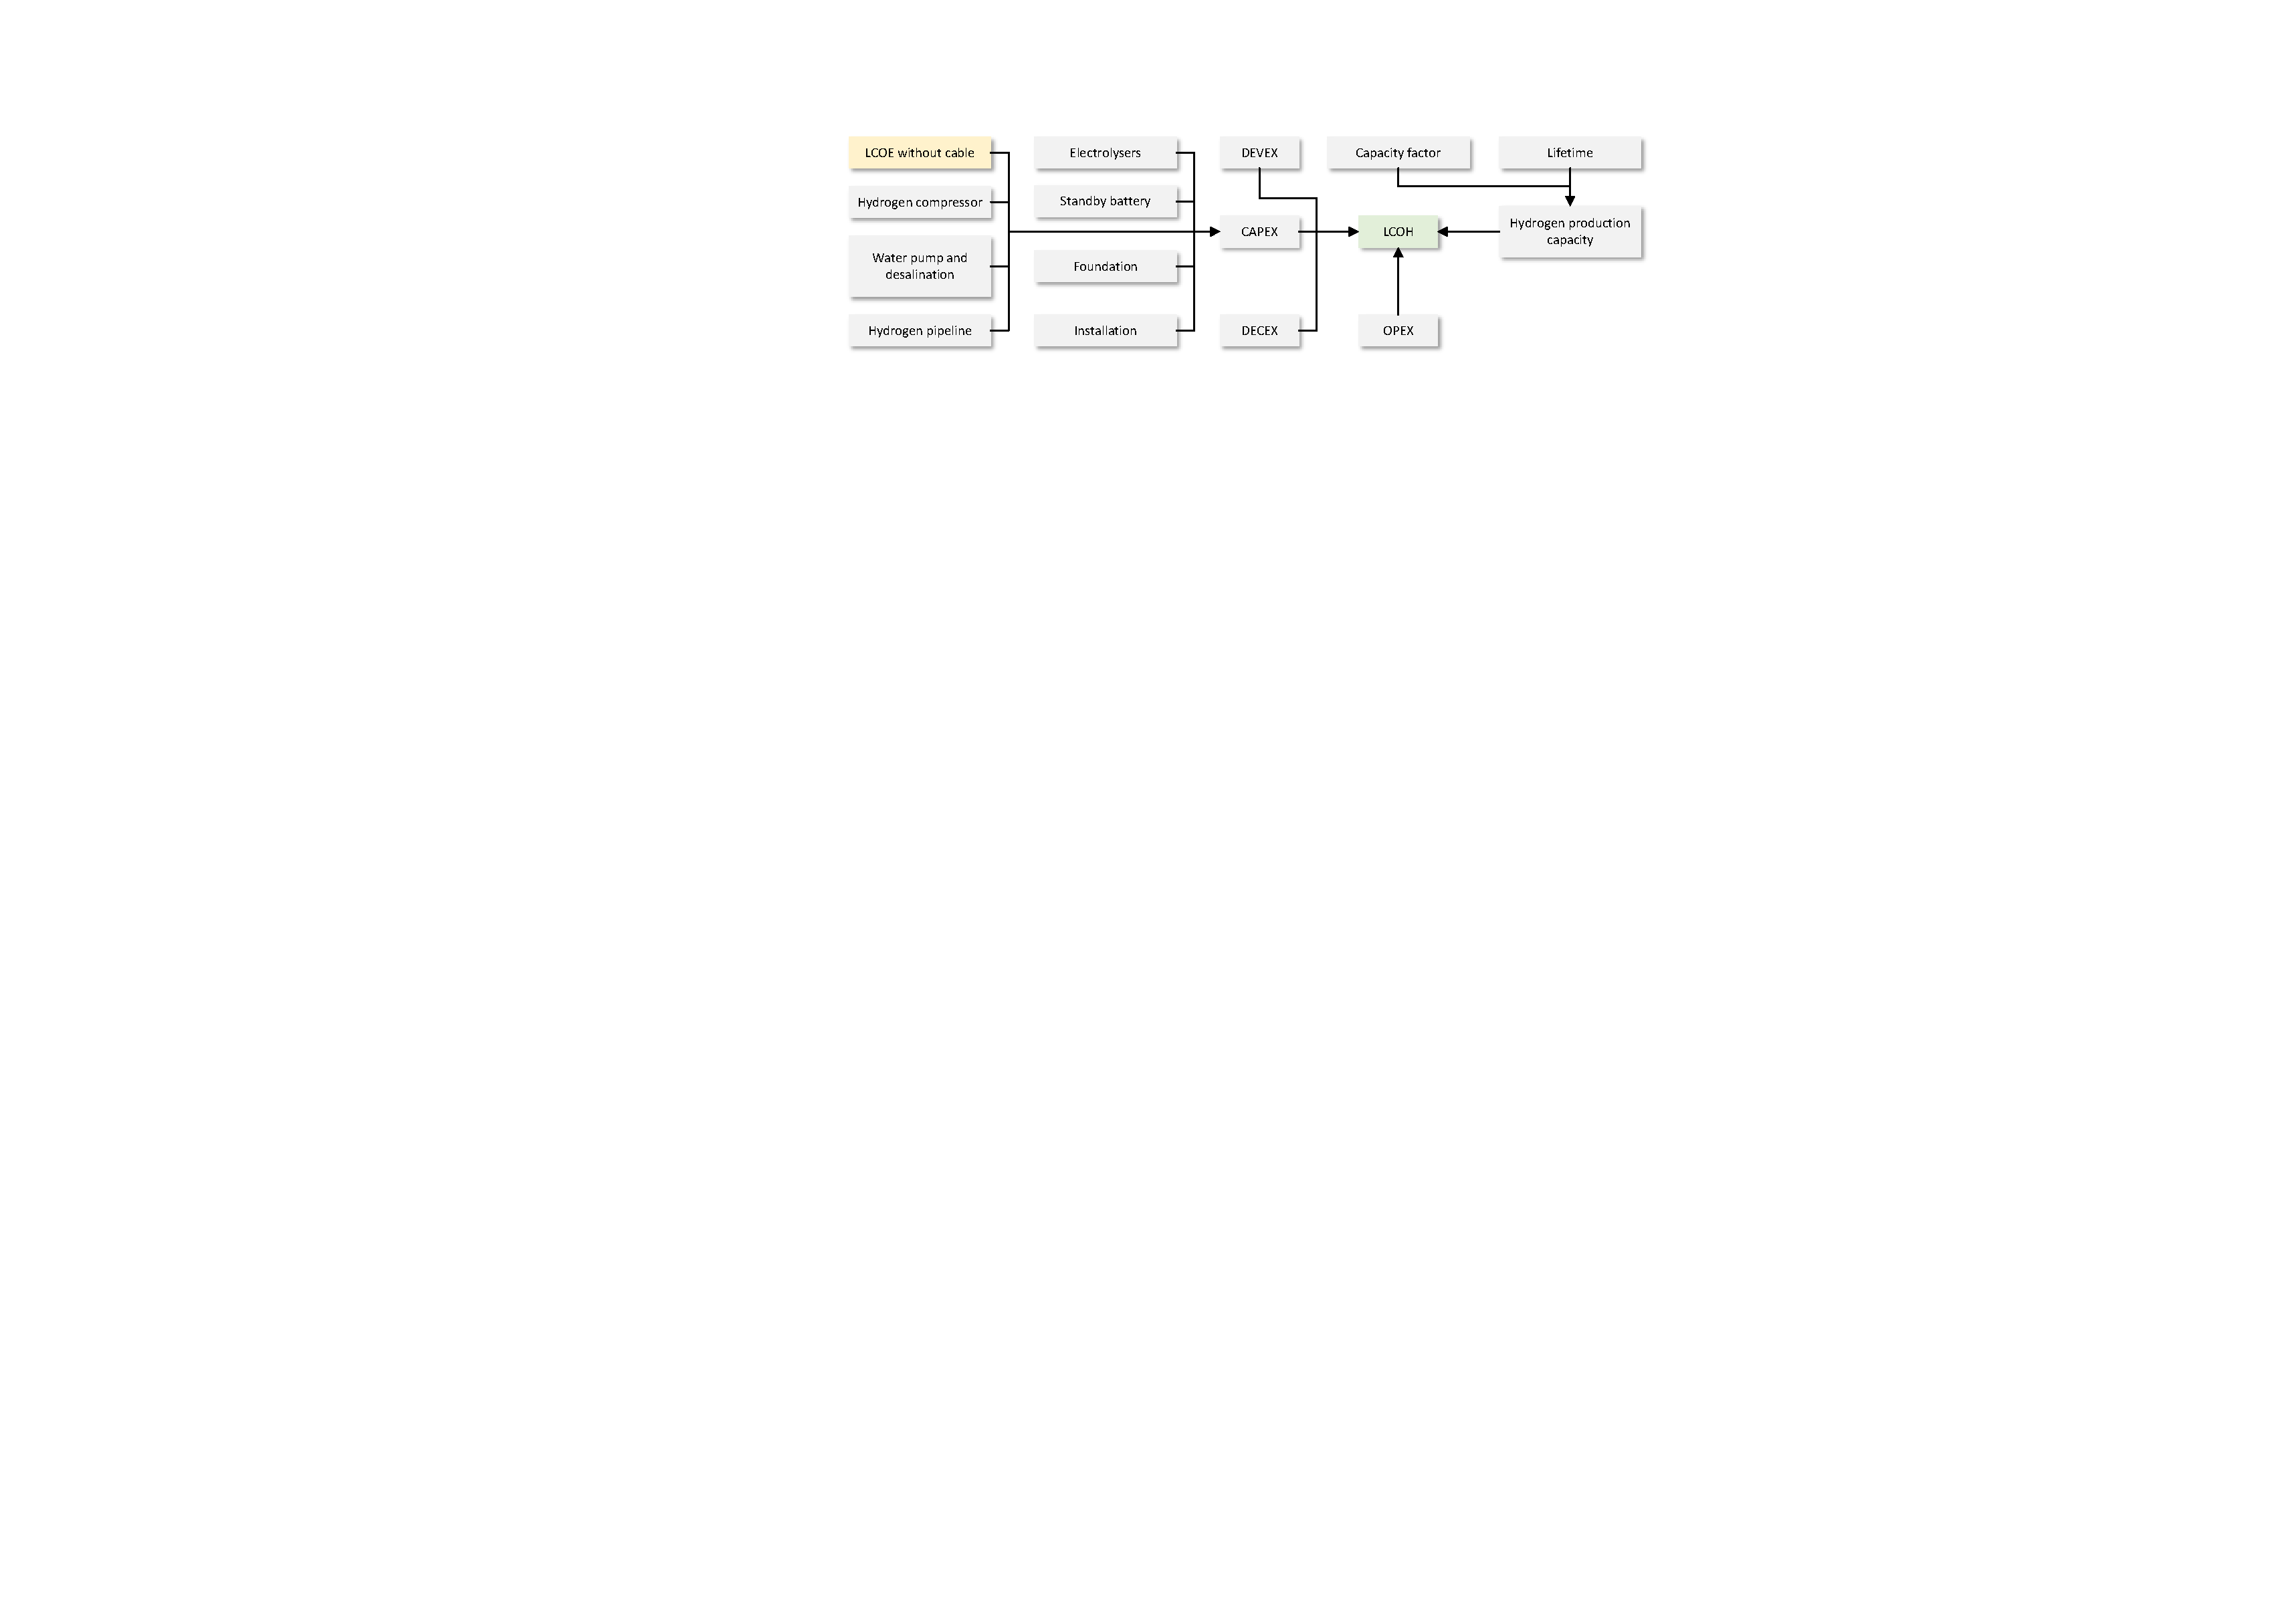
\includegraphics[width =1\columnwidth]{figs/fig LCOH structure.pdf}
    \caption{Structure of LCOH}
    \label{fig lcoh structure}
\end{figure}

The calculation structure of LCOH is shown in Fig. \ref{fig lcoh structure}. The calculation formulation is similar to (\ref{eq LCOE calculation}), but with some additional system components and corresponding expenditures.

In the offshore electrolysis platform, several components consume the energy from offshore wind, including the water pump, desalination system, electrolysis, hydrogen compressor, and standby battery. Their energy consumption can be modelled by:
\begin{gather}
    P^{el} \eta^{el} = Q^{hy} HV^{hy}
\label{eq electrolyser efficiency} \\
    P^{wpd} = \eta^{wpd} M^{water}
\label{eq electricity consumption water pump desal}    \\
    P^{cp} = \eta^{cp} Q^{hy} \left( (p^{hy,high}/p^{hy,low})^{Z^{hy}(1-1/\beta^{cp})}-1 \right)
\label{eq electricity consumption compressor}    \\
    P^{bt} = (1-\eta^{bt}) UL^{bt} (P^{el} + P^{wp} + P^{cp})
\label{eq battery loss}    \\
    P^{bt} + P^{el} + P^{wp} + P^{cp} = P^{owf,rated} \times CF
\label{eq electricity consumption total}
\end{gather}
where (\ref{eq electrolyser efficiency}) denote the energy conversion efficiency of electrolysis process;  (\ref{eq electricity consumption water pump desal}) denote that the power consumption of water pump/desalination system is proportional to the mass of water it processes; (\ref{eq electricity consumption compressor}) calculates the power consumption of compressor \cite{bao2019multi}; (\ref{eq battery loss}) evaluate the average power loss during the utilization of batteries; (\ref{eq electricity consumption total}) denote the total power consumptions of all components add up to the electricity generation of the wind farm; $P^{el}$, $P^{wpd}$, $P^{cp}$, and $P^{bt}$ represent the power consumption (loss) of electrolyser, water pump/desalination system, compressor, and battery, respectively; $\eta^{el}$, $\eta^{wpd}$, $\eta^{cp}$, and $\eta^{bt}$ are the efficiencies of electrolyser, water pump/desalination system, compressor, and battery, respectively; $Q^{hy}$ is the gas flow rate of hydrogen production in standard temperature and pressure condition; $HV^{hy}$ is the heat value of hydrogen; $M^{water}$ is the mass of water being processed; $p^{hy,low}$ and $p^{hy,high}$ are the low and high hydrogen pressure values before/after compression; $Z^{hy}$ is the compressibility factor of hydrogen; $\beta^{cp}$ is the specific heat ratio; $UL^{bt}$ is the utilization rate of battery.

By solving the above equation set, the maximum volume of hydrogen production of this OWF can be obtained. Then, the LCOH can be calculated as:
\begin{gather}
    LCOH = \frac{DEVEX + CAPEX + \sum_{t \in \mathcal{T}} OPEX_t (1+r)^{-(t-1)} + DECEX^{T-1}}
   {8760 Q^{hy} HV^{hy} \times CF \times LF \times T}
\end{gather}

Similar to the LCOE, the total expenditure of hydrogen production includes DEVEX, CAPEX, OPEX, and DECEX. The DEVEX, and part of CAPEX, OPEX, and DECEX, have been calculated in LCOE, and therefore, we focus on calculating the additional cost in this subsection.

\begin{table}[]
\centering
\caption{Offshore hydrogen system costs \cite{OffshoreWindandHydrogen, Offshorewindtogreen}}
\label{tab offshore hydrogen system cost}
\begin{tabular}{llll}
\hline
Capital cost                                                                                                    & Cost in 2030 & Cost in 2040 & Cost in 2050 \\ \hline
Alkaline electrolyser ($10^3$ \texteuro/MW)                       & 625          & 400          & 300          \\
Hydrogen compressor ($10^3$ \texteuro/MW)                         & 3.86         & 2.69         & 2.34         \\
Battery ($10^3$ \texteuro/MW)                                       & 56.39        & 41.54        & 22.58        \\
Water desalination ($10^3$ \texteuro/MW)                            & 1.4          & 0.936        & 0.234        \\
Platform ($10^3$ \texteuro/MW)                                      & 232.13       & 195.98       & 130.45       \\
System replacement ($10^3$ \texteuro/MW)                            & 10.96        & 21.11        & 11.49        \\
Pipeline ($10^3$ \texteuro/(km $\times$ inch)       & 34.74        & 31.42        & 28.41        \\ \hline
\multicolumn{2}{l}{Operation   \& maintenance cost}                                                                               &              &              \\ \hline
Alkaline electrolyser ($10^3$ \texteuro/MW/year)                  & 12.5         & 8            & 6            \\
Hydrogen compressor ($10^3$ \texteuro/MW/year)                   & 0.117        & 0.0819       & 0.0351       \\
Battery ($10^3$ \texteuro/MW/year)                                 & 1.4          & 1.04         & 0.56         \\
Water desalination ($10^3$ \texteuro/MW/year)                    & 0.0468       & 0.0234       & 0.0117       \\
Platform ($10^3$ \texteuro/MW/year)                                & 2.92         & 2.92         & 2.92         \\
Pipeline ($10^3$ \texteuro/(km $\times$ inch/year) & 1.0423       & 0.9427       & 0.8525       \\ \hline
\end{tabular}
\end{table}

The capital and operation\&maintenance costs of components, including Alkaline electrolyser, hydrogen compressor, etc., are presented in Table \ref{tab offshore hydrogen system cost}. The cost of the hydrogen pipeline is calculated according to the minimum distance between the substation and onshore gas buses, similar to (\ref{eq distance to power bus}). The maintenance and installation costs are further normalised using similar equations in the OWF project in the last section, which is further related to the distance to the nearest port. The decommissioning expenditure is taken as a similar proportion to the installation cost. 
% Moreover, the produced oxygen during the electrolysis process is considered a by-product and sold to onshore consumers (such as hospitals) \cite{song2021production}.

\subsection{Route 3: ammonia production}

In this route, we further consider the CAPEX, OPEX, and DECEX of Air separation and Haber–Bosch reactor, which is additional equipment for the ammonia production process. The cost is calculated based on \cite{gonzalez2024techno}.

\begin{figure}
    \centering
    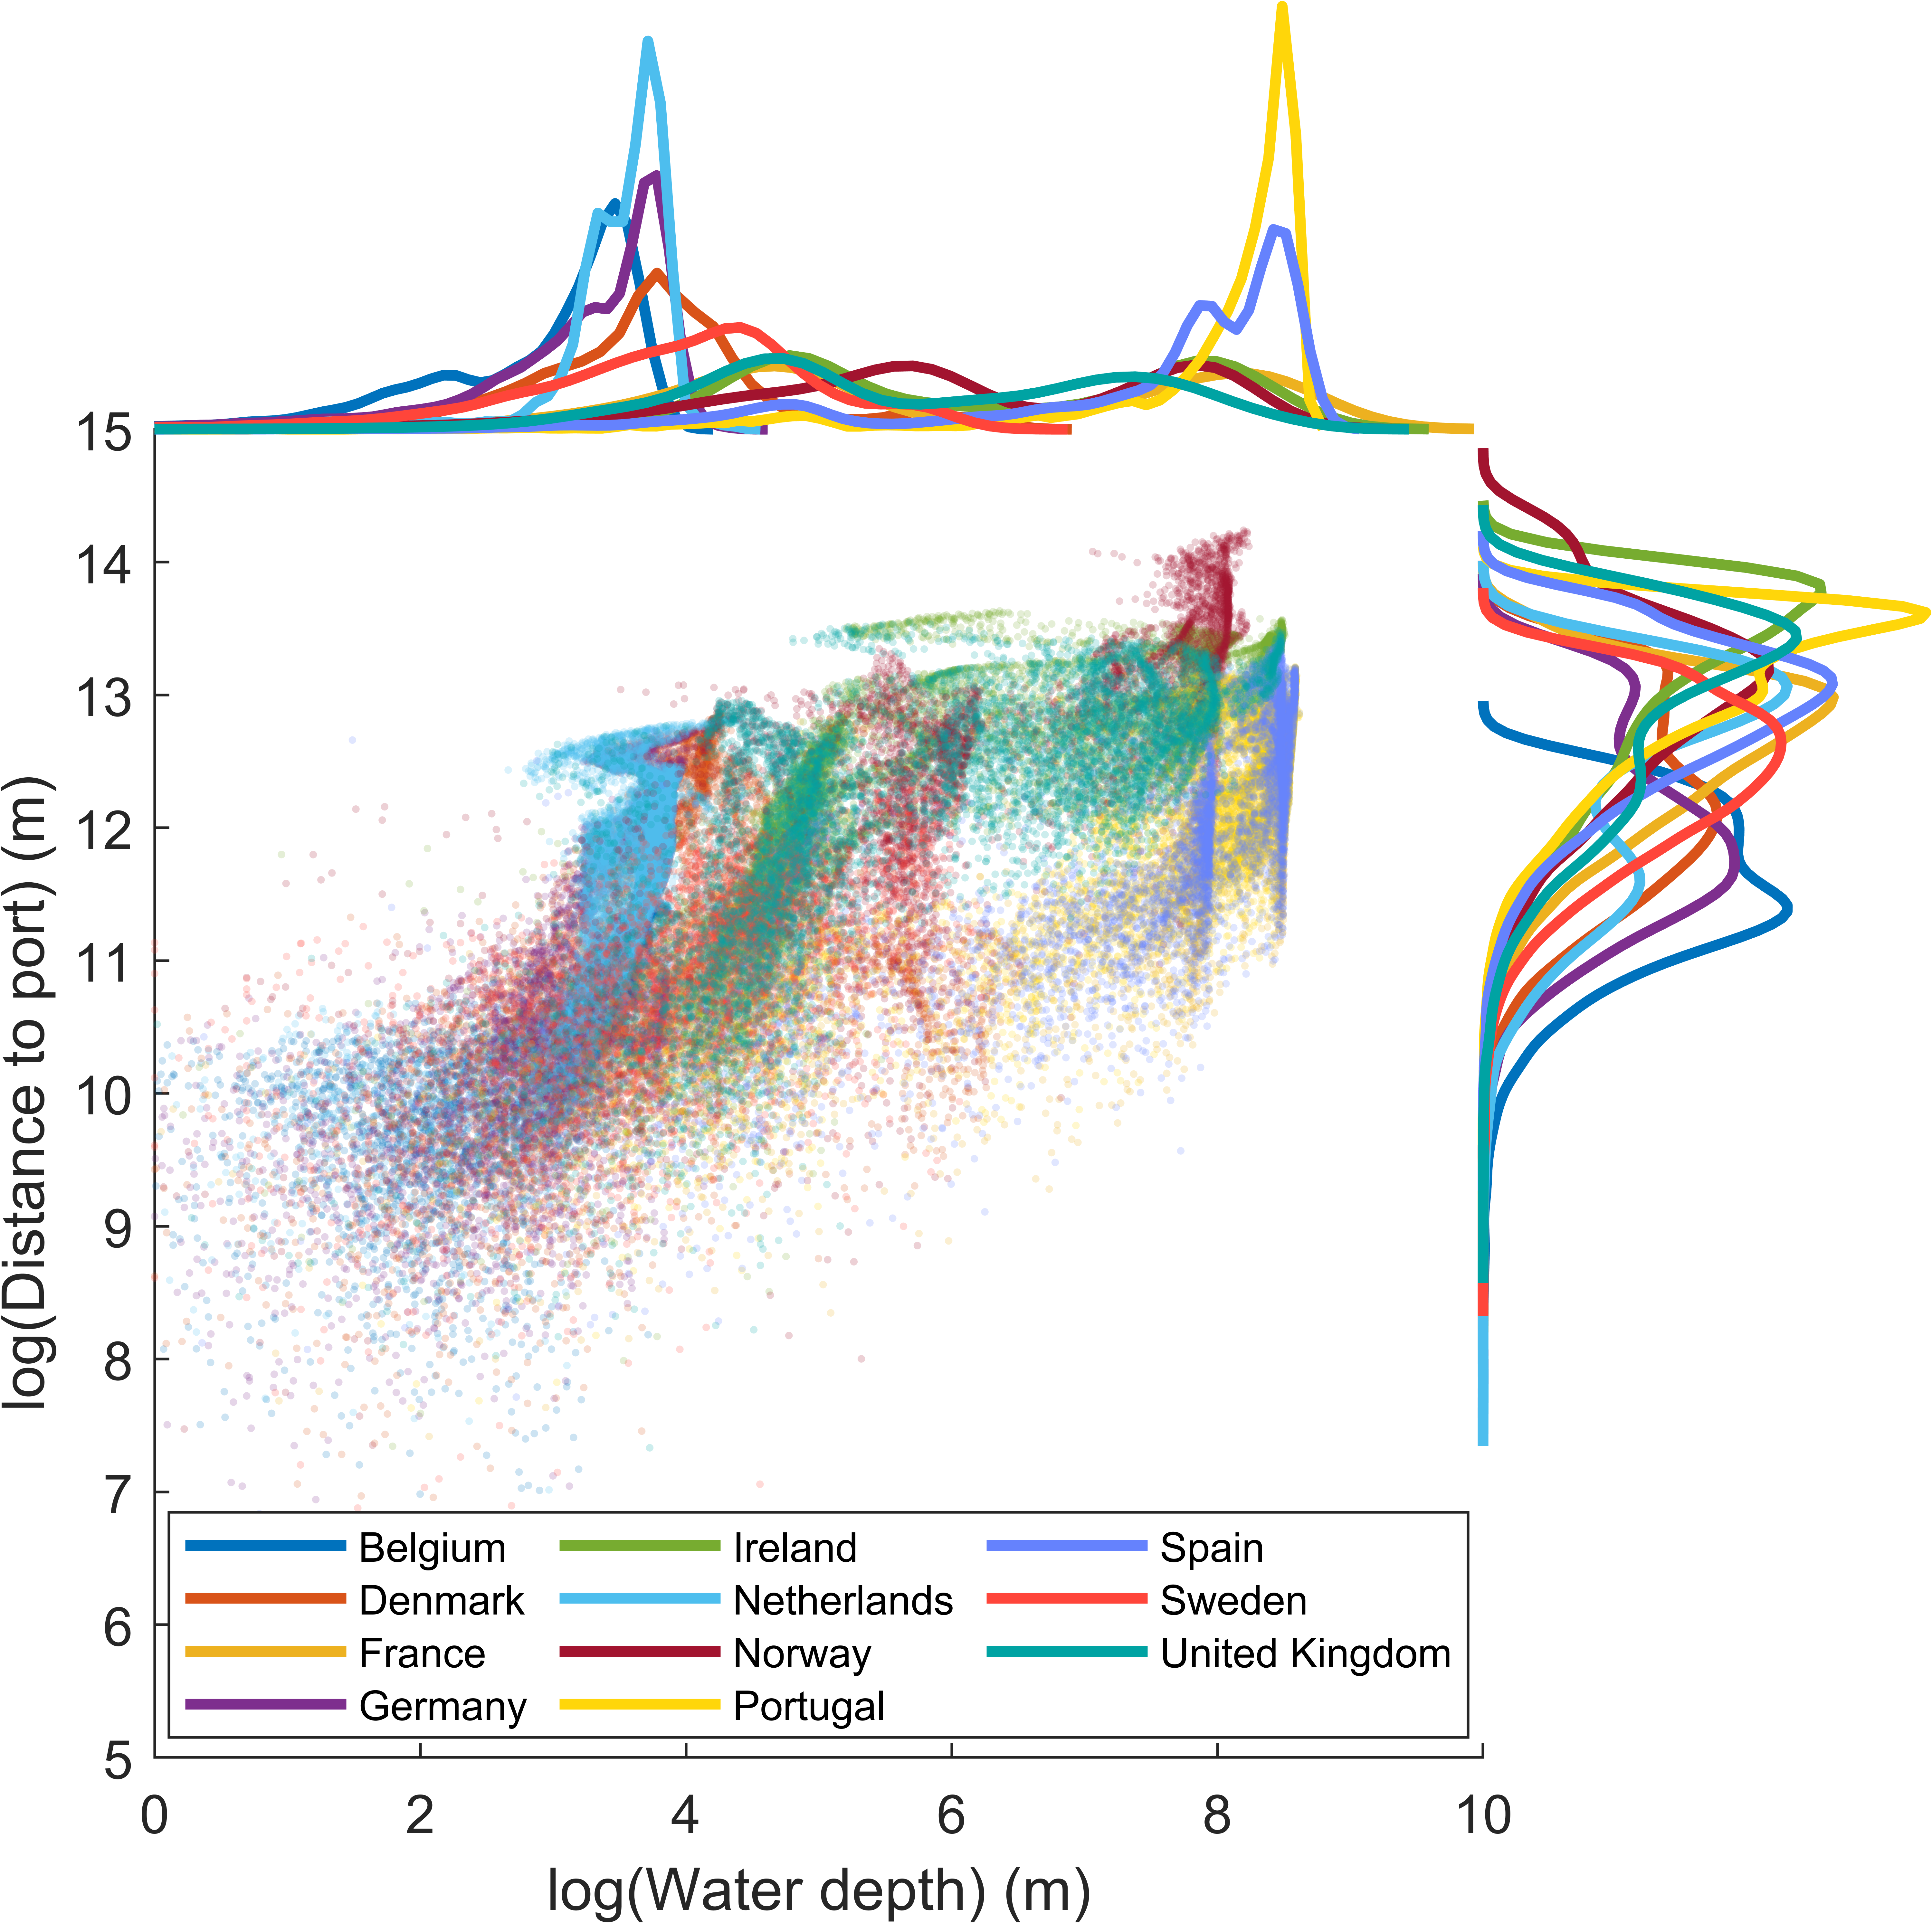
\includegraphics[width =1\columnwidth]{figs/fig distribution of water depth and distance to port.png}
    \caption{Probability distributions of water depths and distance to ports in major countries. In the centre is the scatter diagram of various offshore wind locations. }
    \label{fig water depth distribution}
\end{figure}

Fig. \ref{fig water depth distribution} compares water depth and distance to the port, which are the two major factors affecting the total construction cost of offshore wind, corresponding to material cost and installation/maintenance cost, respectively. We notice that different countries are distributed differently. For example, Belgium is on the left-bottom because all the potential offshore locations in its EEZ both have shallower water and closer distance; While the potential OWF locations in Spain, Norway, etc., on the contrary, have relatively deeper water depths and are more distant. Thus, it can be estimated that these countries may have higher levelized costs for electricity, hydrogen, and ammonia.

\subsection{Cost supply curve and trends in the future}

Based on the LCOH map, to derive the cost-supply curve of hydrogen for each country, the power density is another important factor, which determines how much capacity can be installed within a given area. Firstly, the wake effect, as analysed in Section 1, sets an upper limit for power density, because sitting wind turbines too close will cause interference to downstream turbines. Secondly, for excluded areas (such as military areas, aquaculture sites, and conservation areas, the power density is set to zero. Moreover, the power density further reduces with the increase of vessel density, to reserve for shipping lanes, as shown in Fig. \ref{fig vessel and power density}. 
As we can see, the marine areas in the south of the North Sea, also belonging to the EEZ of Belgium, France, etc., have busy shipping lines. Therefore, though the water depth and distance are in favourable conditions, the quantity of low-cost hydrogen may be limited due to the lower power density. 
The power density in each EEZ is fitted into the probability density curve in the right part of Fig. \ref {fig vessel and power density}. As we can see, for most of Belgium's EEZ area, the power density is around 2.5-3.5 $MW/km^2$ due to the busy shipping lines. Denmark, Germany, and the Netherlands, similarly, have a similar situation to Belgium. In contrast, in Ireland and the UK, due to the sparse shipping lines, especially on the west coasts, the power densities are higher and the modes are distributed around 4-5 $MW/km^2$.

\begin{figure}
    \centering
    \includegraphics[width = 0.99\columnwidth]{figs/fig vessel density and power density.png}
    \caption{Vessel density and power density. On the left is the vessel density. On the right is the probability density of power density for each country's EEZ.}
    \label{fig vessel and power density}
\end{figure}

\begin{figure}
    \centering
    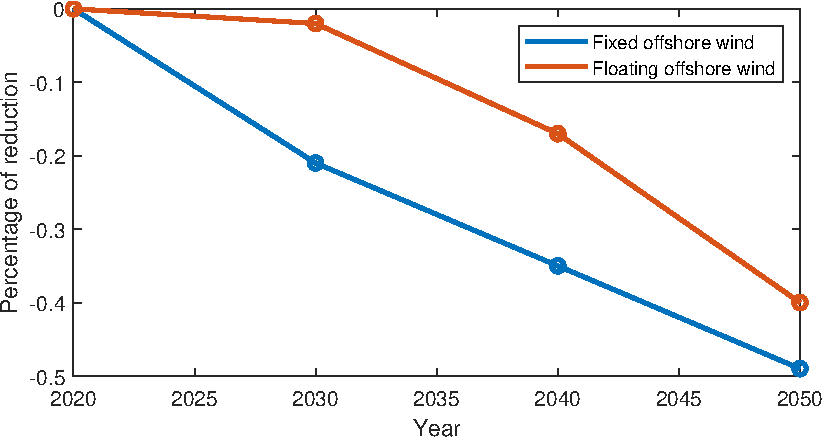
\includegraphics[width = 0.8\columnwidth]{figs/fig cost reduction.pdf}
    \caption{Cost reduction of fixed and floating offshore wind}
    \label{fig cost reduction}
\end{figure}

Considering the potential cost reduction in LCOE \cite{wiser2021expert} and capital cost (as indicated by Table. \ref{tab offshore hydrogen system cost}, the hydrogen supply curves in 2030, 2040, and 2050 can be derived. As shown in Fig. \ref{fig cost reduction}, compared with the cost in 2020, the fixed and floating wind costs can be reduced by 49\% and 40\%, respectively.

\begin{figure}
    \centering
    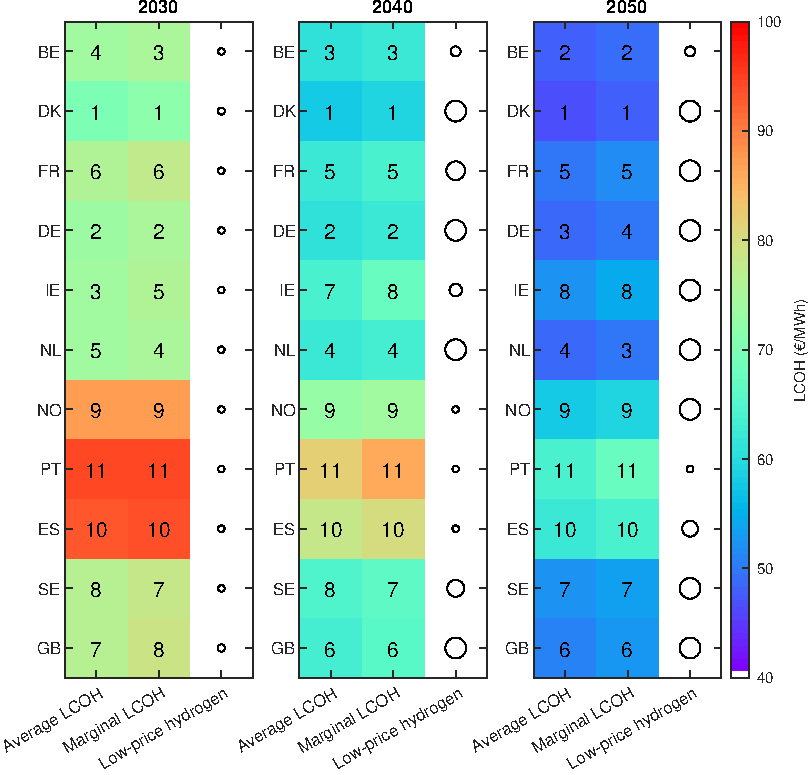
\includegraphics[width = 0.8\columnwidth]{figs/fig_cost_table.pdf}
    \caption{\textbf{Cost-competitiveness of offshore green hydrogen among major countries and with blue hydrogen.} Rank indicates the average or marginal LCOH rank among the 11 studied countries. Marginal means the LCOH at the policy-constrained offshore capacity of that country in the corresponding year. Average means the capacity-weighted average LCOH across the offshore capacity in the corresponding year. Low-price hydrogen means the hydrogen production capacity with production cost below the upper bound of blue hydrogen. The smallest and largest circles indicate 0 and $>$100 GW, and intermediate circle sizes indicate capacities between these values.}
    \label{fig supplementary cost rank}
\end{figure}

\section{Domestic energy system optimisation model}

\begin{figure}
    \centering
    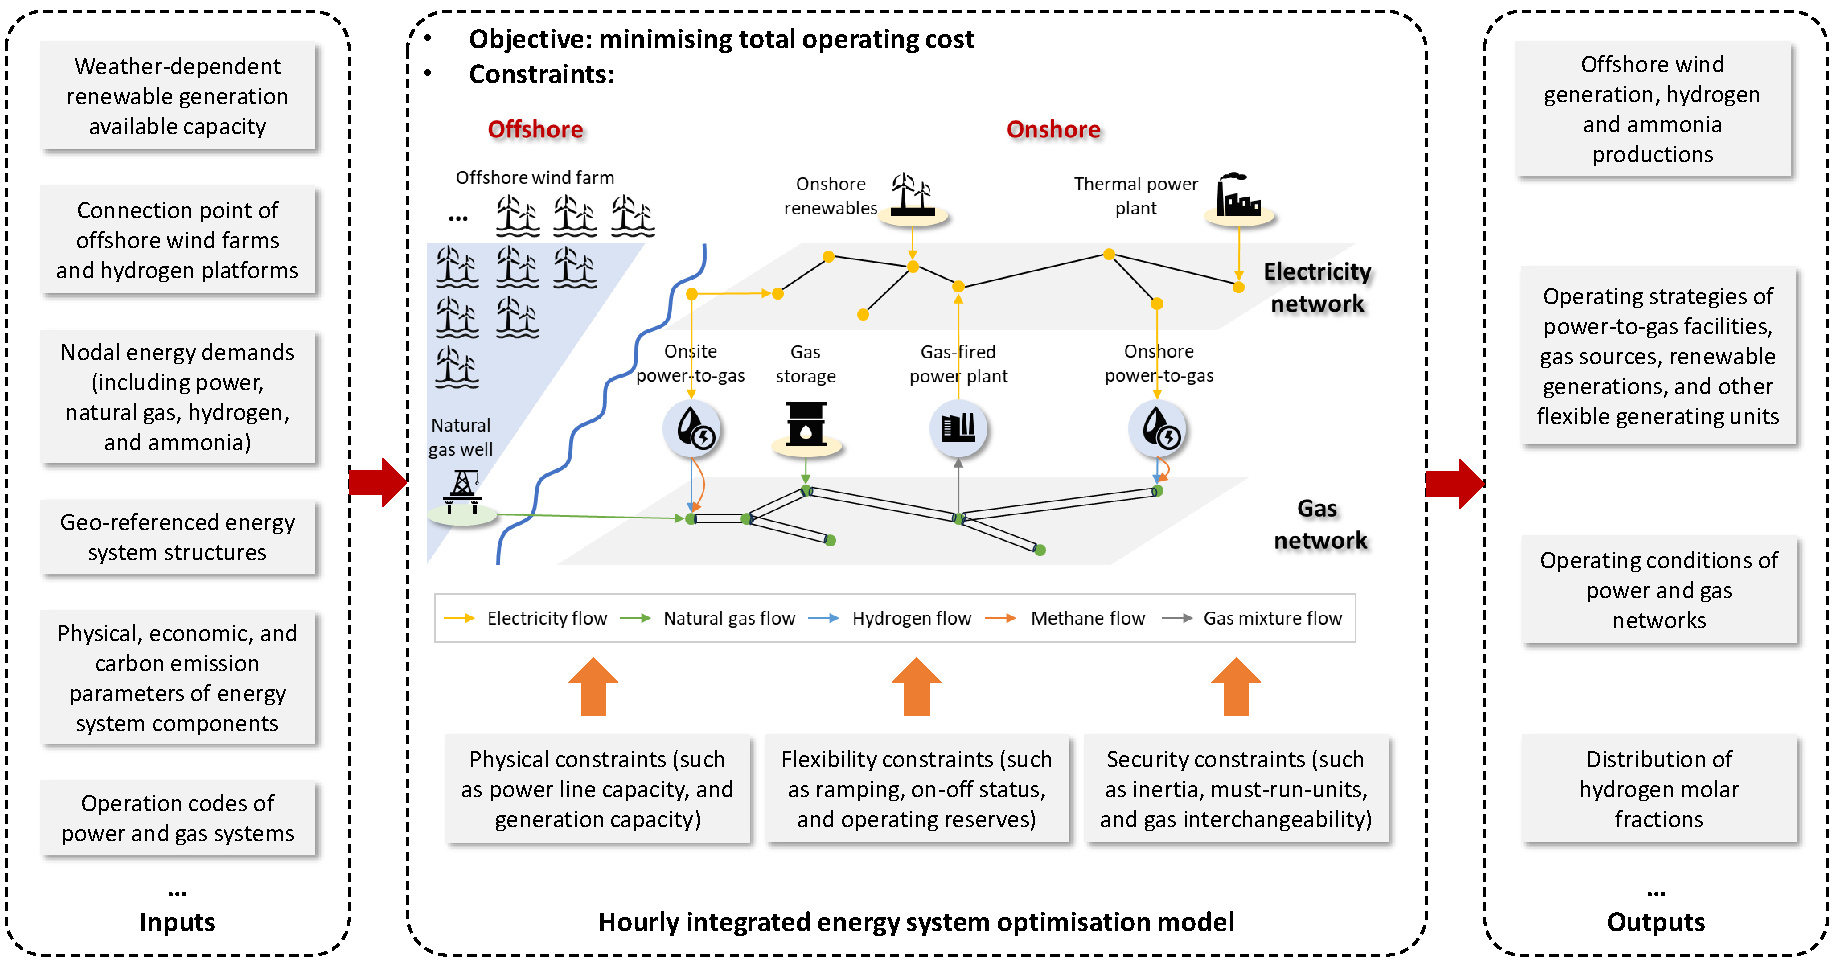
\includegraphics[width = 0.99\columnwidth]{figs/fig optimization structure.pdf}
    \caption{Framework of integrated energy systems optimisation model}
    \label{fig optimization framework}
\end{figure}

In this section, we illustrate the carbon emission mitigation potential for Ireland Island domestic use if offshore wind and hydrogen/ammonia production are integrated as much as possible, as well as its cost.
An integrated energy system optimal operation model is developed, and its framework is shown in Fig. \ref{fig optimization framework}. 
The optimisation is implemented on the basis of hourly time resolution for one year, and $0.1^{\circ}\times 0.1^{\circ}$ longitude and latitude grid spatial resolution for all Ireland offshore wind assessment areas. 
All-Ireland Island energy systems (including the power and gas systems in the Republic of Ireland and Northern Ireland) are within the scope of this study. The power and gas systems are tightly coupled by gas-fired power plants and power-to-gas facilities to enable a bidirectional energy exchange and expand the flexible operating regions. Hydrogen network transportation at different generation levels (also known as hydrogen blending) is considered in the future scenarios in 2030, 2040, and 2050.

The objective of the optimisation problem is to minimise the total operating cost $C^{op}$ during the daily scheduling and operation, including the power system cost (start-up/shut-down cost, fuel cost), and gas system cost (gas supply cost):
\begin{align}
    C^{op} & = \sum_{h \in \mathcal{H}} \bigg( \sum_{i \in \mathcal{I}^e} \sum_{g \in \mathcal{G}_i} u^{on}_{i,g,h} (a_{i,g} P_{i,g,h}^2 + b_{i,g} P_{i,g,h} + c_{i,g}) + u_{i,g,h}^{up} \rho^{up}_{i,g}
    \notag \\
    & + \sum_{i \in \mathcal{I}^g} \rho_{i}^{gs} Q_{i,h}^{gs} \bigg)
\end{align}
where $h$, $i$, and $g$ are the indices for hours, electricity/gas nodes, and generators, respectively; $\mathcal{H}$, $\mathcal{G}$, $\mathcal{I}^e$, and $\mathcal{I}^g$, are the set of hours, generators, electricity nodes, and gas nodes, respectively; $u^{on}_{i,g,h}$ is the status of the generator $g$ at node $i$ in hour $h$, where 1 means on, and 0 means off; $u_{i,g,h}^{up}$ is the start-up action of generators, where 1 means the action is taken, and 0 indicates otherwise;
$a_{i,g}$, $b_{i,g}$, and $c_{i,g}$ are the cost coefficients of generators, which are related to the types and prices of the fuel and heat efficiency obtained from the Single-Electricity-Market (SEM) Committee \cite{SEMPLEXOS}; These parameters are provided in the forms of piecewise functions, which are fitted into quadratic form for convex optimization; $P_{i,g,h}$ is the power output of generator; $\rho^{up}_{i,g}$ is the start-up cost; $\rho_{i}^{gs}$ is the natural gas purchasing price; $Q_{i,h}$ is the flow rate of gas supply.

\subsection{Power system model}

The schematic diagram of All-Ireland's power system is presented in Fig. \ref{fig Ireland power system}. Until Jan 2022, it had 370 over-110 kV buses,  686 branches, and 155 onshore transmission-connected generators, with a total generating capacity of 19.55 GW. The daily electricity peak demands from now to 2032
are predicted by A bottom-up approach in EirGrid’s Ten-Year
Generation Capacity Statement\cite{GenerationCapacity}. It covers the forecasting values from now to 2032 in typical seasonal scenarios (winter, summer, and spring-autumn). Considering the increasing trend of annual power demand is steady, the Autoregressive Integrated Moving Average (ARIMA) is used to fill the missing values between 2033 and 2050. 15-minute-resolution electricity and gas demand curves are used for daily operational analysis. They are obtained from EirGrid’s smart grid dashboard and the Gas Network Ireland data dashboard in different seasonal scenarios \cite{SmartGridDashboard, GasconsumptionbyMarketSector}.

\begin{figure}
    \centering
    
\includegraphics[width = 0.99\columnwidth]{figs/fig ireland power system2.pdf}
    \caption{Transmission system 400 kV, 275 kV and 110 kV, January 2022 \cite{AllIslandTenYear}}
    \label{fig Ireland power system}
\end{figure}

(1) Generators

According to different fuels used in the generation, the generators in Ireland's power systems include coal, gas, gas oil, waste, peat, hydro, wind, and solar, and detailed technical, economic, and carbon-emission-related data can be found from Single-Electricity-Market (SEM) Committee and EirGrid \cite{SEMPLEXOS, AllIslandTenYear}. The generators can be divided into three categories: non-gas fossil fuels, gas, and renewable generations. The fuel supplies of the first category depend on their own supply chain, which is considered steady. Therefore, the capacity constraints during the operation can be written as (\ref{eq nongas generator capacity}); The fuel supply of the second category depends on the operating status of the gas system, which can be written as (\ref{eq gas generator capacity}); The actual dispatchable capacity of the third category is always lower than the designed rated power, depending on the weather condition (wind or solar). Therefore, their capacity constraints can be written as in (\ref{eq renewable generator capacity}). The weather conditions (wind speed and solar radiation) are also obtained from the ERA-5 dataset \cite{ERA5}. (\ref{eq generator on-off}) is the on-off constraint of generators.
\begin{gather}
    u_{i,g,h}^{on} P_{i,g}^{min} \leq P_{i,g,h} \leq u_{i,g,h}^{on} P_{i,g}^{max}, g \in \mathcal{G}_i^{coal,gasoil,waste,peat}
\label{eq nongas generator capacity} \\
    u_{i,g,h}^{on} P_{i,g}^{min} \leq \eta_{i,g}^{gpp} GCV^{ng} \sum_{c \in \mathcal{C}} Q_{i,g,h,n}^{gpp} \leq u_{i,g,h}^{on} P_{i,g}^{max}, g \in \mathcal{G}_i^{gas}
\label{eq gas generator capacity} \\
    u_{i,g,h}^{on} P_{i,g,h}^{min} \leq P_{i,g,h} \leq u_{i,g,h}^{on} P_{i,g,h}^{max}, g \in \mathcal{G}_i^{wind,solar,hydro}
\label{eq renewable generator capacity} \\
    u_{i,g,h}^{on} - u_{i,g,h-1}^{on} = u_{i,g,h}^{up} - u_{i,g,h}^{dn}, \ u_{i,g,h}^{up} + u_{i,g,h}^{dn} \leq 1, \ u_{i,g,h}^{on}, u_{i,g,h}^{up}, u_{i,g,h}^{dn} \in \{0,1\}
\label{eq generator on-off} 
\end{gather}
where $u_{i,g,h}^{on}$ is the on-off status of the unit, where 1 and 0 represent on and off, respectively; $u_{i,g,h}^{up}$ and $u_{i,g,h}^{dn}$ are the indicators for start-up and shut-down actions, respectively; $P_{i,g}^{min}$ and $P_{i,g}^{max}$ are the lower and upper bounds for the power output of generator $g$ at electric node $i$; $P_{i,g,h}$ is the power output of generator $g$ at node $i$ at hour $h$; $\mathcal{G}_i^{coal}$ is the set of the coal-fired power plant at node $i$, and others with different superscripts are similar; $\eta_{i,g}^{gpp}$ is the efficiency of the gas-fired generating unit converting gas energy to electric power; $GCV^{ng}$ is the gross caloric value of natural gas; $Q_{i,g,h,n}^{gpp}$ is the gas consumption of the gas-fired generating unit for gas component $n$ (in this case, we assume the gas composition of natural gas supply for Ireland is consistent, and therefore, $n=1,2$ represents natural gas and hydrogen, respectively).

The generator's ramping flexibility is the main assurance against the fluctuation of offshore/onshore wind and solar power. It is constrained by the maximum ramping speed of generators. Usually, the ramping services are provided by non-renewable units, which can be written as:
\begin{gather}
    -RP_{i,g}^{max} \leq P_{i,g,h} - P_{i,g,h-1} \leq RP_{i,g}^{max}, g \in \mathcal{G}_i^{coal,gasoil, waste, peat, gas, hydro}
\end{gather}
where $RP_{i,g}^{max}$ are the maximum ramping rate of the generator.

(2) DC power flow constraints

For transmission-level power systems, the resistance of power lines is much smaller than reactance. Therefore, the DC model is accurate enough for power flow calculations, which is widely adopted by worldwide system/market operators \cite{stott2009dc}. (\ref{eq dc power flow cons}) is describes the voltage angle drop along the power line with respect to transmission electric power; (\ref{eq active power balance}) is the nodal power balance; The voltage angles and power flow should be limited as in (\ref{eq voltage angle cons}) and (\ref{eq line flow cons}):
\begin{gather}
    \theta_{i,h} - \theta_{j,h} = X_{ij} pf_{ij,h}
\label{eq dc power flow cons}\\
    \sum_{g \in \mathcal{G}}{P_{i,g,h}}
    + P^{ic}_{i,h}
    - \sum_{g \in \mathcal{G}_i^{ptg}}{P_{i,g,h}^{ptg}}
    - P_{i,h}^{d}
    - \sum_{j \in \mathcal{J}_i}{pf_{ij,h}} = 0
\label{eq active power balance} \\
    \theta^{min} \leq \theta_i \leq \theta^{max}
\label{eq voltage angle cons}    \\
 - pf_{ij}^{max} \leq pf_{ij,h} \leq pf_{ij}^{max}
\label{eq line flow cons}
\end{gather}
where $\theta_{i,h}$ is the voltage angle; $X_{ij}$ is the reactance of power line connecting node $i$ and $j$; $\mathcal{g}_i^{ptg}$ is the set of PTG; $P_{i,g,h}^{ptg}$ is the electric power consumption of PTG; $P_{i,h}^{d}$ is the nodal electricity demand; $pf_{ij,h}$ is the power flow in power line $ij$; $\mathcal{J}_i$ is the set of node connected to node $i$; $\theta^{min}$ and $\theta^{max}$ are lower and upper bounds for voltage angle, respectively; $pf_{ij}^{max}$ is the capacity of power line $ij$.

(3) Interconnectors

Currently, Ireland island has two interconnectors with the UK, i.e., Ireland and Wales (EWIC) and Northern Ireland and Scotland (Moyle) \cite{RealTimeSystemInformation}. During the operation, they can be regarded as two equivalent generators, where the generating and ramp rate are the transmission capacity and ramp rate of the interconnectors (except that the capacity can be negative), and the marginal cost is set to the auction results of interconnectors \cite{InterconnectorRequirement}:
\begin{gather}
    - P^{ic,max}_{i,h} \leq P^{ic}_{i,h} \leq P^{ic,max}_{i,h}
\label{eq interconnector capacity}\\
    - RP^{ic,max}_{i,h} \leq P^{ic}_{i,h} - P^{ic}_{i,h-1} \leq RP^{ic,max}_{i,h}
\label{eq interconnector ramp}
\end{gather}
where $P^{ic}_{i,h}$ is the flow-in power of the interconnector that connects to node $i$; $P^{ic,max}_{i,h}$ is the capacity of the interconnector; $RP^{ic,max}_{i,h}$ is the maximum ramping speed.
Besides the two existing interconnections, Ireland is planning to build a 700 MW Celtic Interconnector with France in the future, in around 2027 \cite{CelticInterconnector}. It will be modelled similarly in future scenarios.

\begin{table}[]
\centering
\caption{Dynamic stability constraints in future scenarios}
\label{tab stability cons}
\begin{tabular}{p{3.9cm}p{2.0cm}p{1.6cm}p{1.6cm}p{1.6cm}}
\hline
\textbf{Constraints}                                                                & \textbf{Values now}              & \textbf{Values in 2030} & \textbf{Values in 2040} & \textbf{Values in 2050} \\ \hline
Inertia                                                                             & 23 GWs                           & 20 GWs                  & 17 GWs                  & 14 GWs                  \\
\begin{tabular}[c]{@{}l@{}}Minimum Number of\\      Conventional Units\end{tabular} & 5 for Ireland and 3 for Northern Ireland            & 3 in total              & 2 in total              & 1 in total              \\
System   Non-Synchronous Penetration                                                & 75 \%                            & 95\%                    & 97\%                    & 99\%                    \\
Regulating Reserve                                                                  & 75 MW for Ireland and 50 MW for Northern Ireland    & /                       & /                       & /                       \\
Primary Operating Reserve                                                           & 75\% Largest Single Infeed (LSI) & 75\% LSI                & 75\% LSI                & 75\% LSI                \\
Secondary Operating Reserve                                                         & 75\% LSI                         & 75\% LSI                & 75\% LSI                & 75\% LSI                \\
Tertiary Operating Reserve 1\&2                                                     & 100\% LSI                        & 100\% LSI               & 100\% LSI               & 100\% LSI               \\
Replacement Reserve                                                                 & 100\% LSI                        & 100\% LSI               & 100\% LSI               & 100\% LSI               \\
Interconnector Ramping Rate                                                         & 10 MW/min      & 15 MW/min                   & 15 MW/min                   & 15 MW/min                   \\ \hline
\end{tabular}
\end{table}

(4) Dynamic stability constraints

According to the operational policy roadmap of EirGrid for 2030, the dynamic stability constraints are evolving with the increasing ability of EirGrid to operate the high-renewable penetrated power systems \cite{OperationalPolicy}. As shown in the Table.\ref{tab stability cons}, the dynamic stability constraints include inertial constraints (\ref{eq inertia}), the minimum number of conventional units (\ref{eq must run units}), System Non-Synchronous Penetration (SNSP) constraints (\ref{eq SNSP cons}), reserve constraints (\ref{eq reserve cons 1}) and (\ref{eq reserve cons 2}), interconnector ramping constraints (\ref{eq interconnector ramp}):
\begin{gather}
    \sum_{i \in \mathcal{I}} \sum_{g \in \mathcal{G}_i} H_{i,g} u_{i,g,h}^{on} \geq H^{min}
\label{eq inertia} \\
    \sum_{g \in \mathcal{G}^{must}} u_{i,g,h}^{on} \geq MUST^{min}
\label{eq must run units} \\
    \sum_{i \in \mathcal{I}} \left( P^{ic}_{i,h} + \sum_{l \in \mathcal{L}^{wind,solar}} P_{i,g,h} \right) \leq SNSP^{min}
\label{eq SNSP cons}\\
    \sum_{i \in \mathcal{I}^e} \sum_{g \in \mathcal{G}} u_{i,g,h}^{on} RP_{i,g,h}^{max} \geq 125 + 3.5 \max \{u_{i,g,h}^{on} P_{i,g}^{max}\}
\label{eq reserve cons 1}\\
    \sum_{i \in \mathcal{I}^e} \sum_{g \in \mathcal{G}} u_{i,g,h}^{on} (P_{i,g}^{max} - P_{i,g,h}) \geq 125 + 3.5 \max \{u_{i,g,h}^{on} P_{i,g}^{max}\}
\label{eq reserve cons 2}
\end{gather}
where $H_{i,g}$ is the inertia of generator; $H^{min}$ is the lower bounds for system inertia; $G^{must}$ is the set of candidate must run units; $MUST^{min}$ is the minimum number of must run unit; $SNSP^{min}$ is the minimum level of SNSP.

\subsection{Gas system model}

\begin{figure}
    \centering
    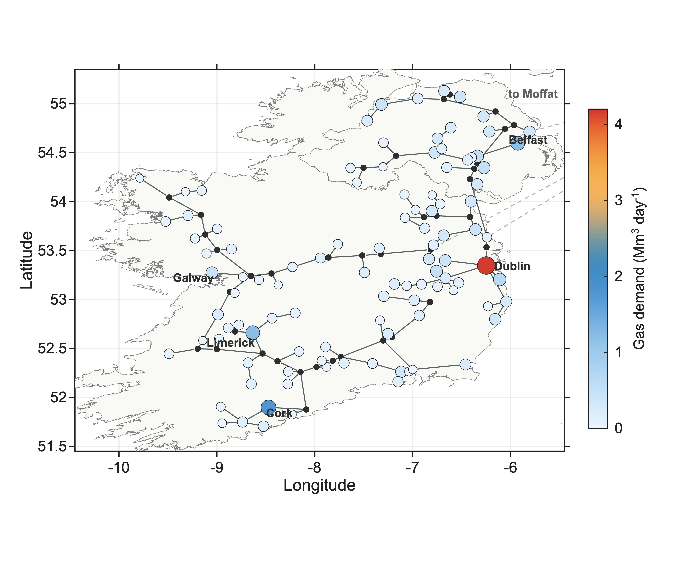
\includegraphics[width = 0.99\columnwidth]{figs/fig ireland gas system.pdf}
    \caption{Gas system in Ireland Island. The gas demand nodes are represented with different colours and sizes, corresponding to different levels of gas demand. Other gas nodes are represented by black dots. Black lines represent the gas pipelines which connect gas nodes.}
    \label{fig Ireland gas system}
\end{figure}

Fig. \ref{fig Ireland gas system} shows the schematic diagram of the Ireland Island gas system. The structure and physical parameters are provided by Gas Network Ireland \cite{NetworkDevelopmentPlan}. It has 144 high-pressure gas buses and gas pipelines for over 16 barg. Currently, there are two major gas suppliers, including one from the UK (Moffat Point), with a maximum capacity of 35 Mm$^3$/day, and another from the northwest of Ireland (Corrib Point) with a maximum capacity of 6.21 Mm$^3$/day. Similar to the power system, the Dublin area has the largest gas consumption. Natural gas generally flows from northeast to southwest.

(1) Gas demand trend

Long-term and high-resolution gas demand is used for analysis. 
The hourly gas demand curve for a year is obtained from the Gas Network Ireland data dashboard \cite{GasconsumptionbyMarketSector}.
The trends of gas demand in the future scenarios are predicted according to the Gas Forecast statement by Gas Network Ireland \cite{GasForecastStatement2022, Irishelectricityandgasdemand}.
The gas demands are mainly from the power generation sector, 
In the power sector, some coal-fired power plants (such as Moneypoint units) may retire in the future and be replaced by natural gas-generating units. In the meantime, with the 80\% renewable generation ambition from the Irish government's Climate Action Plan, the increasing renewable generation will replace the gas-fired generation. For industrial and commercial sectors, the gas demand will continue to increase in proportion to new connection numbers and Gross Domestic Product (GDP). For the residential sector, because Ireland's Climate Action Plan has explicitly banned the new installation of decentralised natural gas boilers from 2023 and replaced them with electric heat pumps, the gas demand will decrease in general. For the transportation sector, with the construction of new compressed natural gas (CNG) stations, the demand for natural gas is expected to grow.
Therefore, in summary, the gas demand will increase in the short term and reach a peak around 2025, and then continue to decrease from then on, as shown in Fig. \ref{fig future gas demand}. 

\begin{figure}
    \centering
    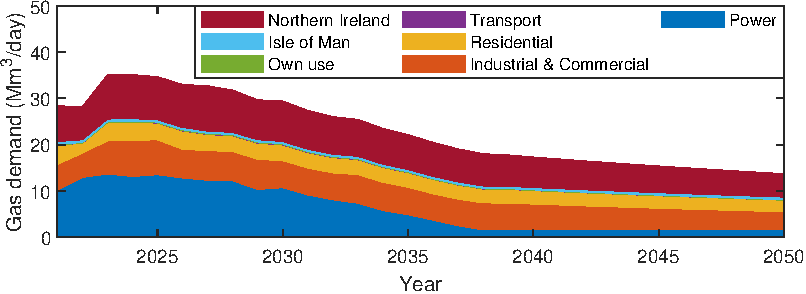
\includegraphics[width = 0.8\columnwidth]{figs/fig future ireland gas demand.pdf}
    \caption{Daily peak gas demand forecast for 2020 - 2050}
    \label{fig future gas demand}
\end{figure}

(2) Gas supply and demand models

Considering the use of alternative gases (hydrogen, biogas, etc.), the gas compositions in the gas system can not be regarded as constant. Seven gas components, which are commonly seen in natural gas, are considered, including methane, ethane, propane, butane, hydrogen, nitrogen, and carbon dioxide. Their gas compositions are denoted as $x_r, (r = 1,2,...,7)$,$\sum_{n \in \mathcal{R}} x_r = 1$, where $r$ and $N$ are the index and set of gas components, respectively. For each different gas source (natural gas, biogas, etc.), they may have different gas compositions. Then, the gas supply of a specific gas component can be calculated by:
\begin{gather}
    Q_{i,g,h,r}^{gs} = Q_{i,g,h}^{gs} x_{i,r}^{gs}
\end{gather}
where $Q_{i,h}^{gs}$ is the capacity of the gas supply at gas node $i$; $x_{i,r}^{gs}$ is the gas composition of the gas supplied from the gas source; $Q_{i,h,r}^{gs}$ is the specific gas flow rate of gas component $r$.

Particularly for PTG, it uses water asa  raw material and consumes electricity to produce hydrogen via the electrolysis process. Then, this process can be expressed as:
\begin{gather}
    Q_{i,g,h}^{ptg} = P_{i,g,h}^{ptg} \eta_{i,g}^{ptg} / GCV^{hy}
\end{gather}
where $Q_{i,g,h}^{ptg}$ is the hydrogen production rate of the PTG; $P_{i,g,h}^{ptg}$ is the power consumption of the PTG; $\eta_{i,g}^{ptg}$ is the electrolysis efficiency; $GCV^{hy}$ is the GCV of hydrogen.

For gas demand, considering different gas compositions, the total heat value of the supplied gas mixtures should match the gas demand. Therefore, we have:
\begin{gather}
    \sum_{r \in \mathcal{R}} GCV_r Q_{i,h,r}^{d} = GCV^{ng} Q_{i,h}^{d}, Q_{i,h,r}^{d} \geq 0
\end{gather}
where $\mathcal{R}$ is the set of gas composition; $GCV_r$ is the GCV of gas component $r$; $Q_{i,h,r}^{d}$ is the gas component $r$ consumed by the gas demand; $GCV^{ng}$ id the GCV of natural gas; $Q_{i,h}^{d}$ is the gas demand expressed in gas flow rate. 

(2) Gas network constraints

The produced gases are transported through pipelines. The physical properties of the gas flowing in a pipeline (gas pressure and gas flow rate) are governed by Weymouth equations \cite{an2003natural}:
\begin{gather}
    p_{i,h}^2 - p_{j,h}^2 = \gamma_{ij} \frac{16 F_{ij} (\rho^{ng})^2 T^{ng} L_{ij}z^{ng}}{\pi^2 D_{ij}^5} {R}_{ij} {Q}_{ij,h}^2
\label{eq gas flow weymouth} \\
     Q_{ij,h} = \sum_{r \in \mathcal{R}} Q_{ij,h,r}
\label{eq gas flow sum, gas constant} \\
    (1-\gamma_{ij})Q_{ij}^{max}/2 \leq [Q_{ij,h}, Q_{ij,h,r}] 
    \leq (1+\gamma_{ij})Q_{ij}^{max}/2
\label{eq capacity pipeline} \\
    p_i^{min} \leq p_{i,h} \leq p_i^{max}
\label{eq pressure limit}
\end{gather}
where $p_{i,h}$ is the gas pressure; $\gamma_{ij,h}$ is the direction of gas flow in pipeline $ij$; $F_{ij}$, $L_{ij}$, and $D_{ij}$ are the friction factor, length, and diameter of the pipeline, respectively; $\rho^{ng}$, $T^{ng}$, and $z^{ng}$ are the gas density, temperature, and compressibility factor of natural gas, respectively; $Q_{ij,h}$ is the gas flow in the pipeline, and $Q_{ij,h,r}$ is the gas flow rate of gas component $r$ specifically; $Q_{ij}^{max}$ is the transmission capacity of the pipeline; $p_i^{min}$ and $p_i^{max}$ are the lower and upper bounds of nodal gas pressure, respectively.

During the transmission, multiple pipelines could be connected to the same gas node. The gases that flow into this node will be mixed evenly first and then distributed to the downstream pipelines. During this process, the nodal balance equations in terms of different gas components should be followed, as in (\ref{eq nodal gas balance}). The gas mixing process is expressed as (\ref{eq gas mixing}).
\begin{gather}
    \sum_{g\in \mathcal{G}_i^{gs}} {Q_{i,g,r}^{s}} + \sum_{l \in \mathcal{G}_i^{ptg}}{Q_{i,g,h,r}^{ptg}}
    + \sum_{j \in \mathcal{J}_i}{\frac{1-\gamma_{ij}}{2} Q_{ij,h,r}} \notag \\
    = \sum_{j \in \mathcal{J}_i}{\frac{1+\gamma_{ij}}{2} Q_{ij,h,r} } + 
    \sum_{l \in \mathcal{G}_i^{gpp}} Q_{i,g,h,r}^{gpp}
    + Q_{i,h,r}^{d}
\label{eq nodal gas balance} \\
    x_{i,r} = \bigg( \sum_{j \in \mathcal{J}_i} {\frac{\gamma_{i,j}-1}{2} Q_{i,j,r}} 
    + \sum_{g\in \mathcal{G}_i^{gs}} {Q_{i,g,r}^{gs}} 
    + \sum_{g\in \mathcal{G}_i^{ptg}} {Q_{i,g,r}^{ptg}} \bigg) / 
\notag \\
    \bigg( \sum_{r \in \mathcal{R}} \bigg( \sum_{j \in \mathcal{J}_i} {\frac{\gamma_{i,j}-1}{2} Q_{i,j,r}} 
    + \sum_{g\in \mathcal{G}_i^{gs}} {Q_{i,g,r}^{gs}} 
    + \sum_{g\in \mathcal{G}_i^{ptg}} {Q_{i,g,r}^{ptg}} \bigg) \bigg)
\label{eq gas mixing}
\end{gather}
where $\mathcal{G}_i^{gs}$ is the set of gas sources in gas node $i$.

(4) Gas security constraints

When hydrogen is blended into the network and the gas composition changes, it may bring gas security issues. For example, appliances are usually designed and
tested at a given pressure with a specific type of gas. They
may not perform satisfactorily if the gas composition changes. The risks of flashback and fire hazards may also increase due to the higher flame speed of hydrogen. Therefore, certain gas security constraints should be imposed on the energy system operation to avoid too much hydrogen injection. According to recently amended Gas Safety (Management) Regulations \cite{GasSafetyRegulations}, the Wobbe index (WI), flame speed factor (FS) (which is additionally introduced to limit the flame speed), relative density, and the molar fraction of hydrogen can serve as indices to regulate gas safety:
\begin{gather}
    RD_{i,k} = \sum_{n \in \mathcal{N}} x_{i,k,n} M_n / M^{air}
\label{eq relative density} \\
    WI_{i,k} = \sum_{n \in \mathcal{N}} x_{i,k,n} GCV_n / \sqrt{RD_{i,k}}
\label{eq WI} \\
    FS_{i,k} = \frac{\sum_{n \in \mathcal{N}}{x_{i,k,n} fs_n }} {AF+5x_{i,k}^{ni}-18.8x_{i,k}^{ox}+1}
\label{eq FS} \\
    0 \leq x_{i,k}^{hy} \leq x^{hy,max}
\label{eq hydrogen fraction limit}\\
    RD_{i,k} \leq  RD^{max}
\label{eq relative density limit}\\
    WI^{min} \leq WI_{i,k} \leq WI^{max}
\label{eq WI limit}\\
    FS^{min} \leq FS_{i,k} \leq FS^{max}
\label{eq flame speed limit}
\end{gather}
where $RD_{i,k}$, $WI_{i,k}$, and $FS_{i,k}$ are the relative density, WI, and FS of the gas mixture at bus $i$ in dispatch interval $k$, respectively; $M_n$ is the molecular weight of gas component $n$; $M^{air}$ is the molecular weight of air; $x_{i,k}^{hy}$, $x_{i,k}^{ni}$, and $x_{i,k}^{ox}$ are the molar fractions of hydrogen, nitrogen, and oxygen in bus $i$ at dispatch interval $k$, respectively; $fs_n$ is the flame speed factor of gas component $n$; $AF$ is the air-fuel ratio; $x^{hy,max}$ and $RD^{max}$ are the upper bounds of hydrogen molar fraction and relative density, respectively; $WI^{min}$, $WI^{max}$, $FS^{min}$ and $FS^{max}$ are the lower and upper bounds of WI and FS, respectively. 

\subsection{Solution method and results in representative scenarios}

Observing the mathematical structure of the optimisation problem formulated above, we find that it is nonlinear and nonconvex, which makes it challenging to obtain a robust solution directly by off-the-shelf solvers. Second-order cone relaxation and advanced sequential programming techniques are used to solve this problem. To see more details, please refer to \cite{wang2023optimal}. After the reformulation, the problem becomes a second-order cone programming problem, which can be solved by commercial solvers such as Gurobi or Mosek. 


\section{International trading model and carbon emission impact analysis}

\subsection{Demand and supply models of hydrogen and ammonia}

International hydrogen and ammonia trading is a critical measure of balancing the country-wide uneven distribution of natural endowment for offshore hydrogen/ammonia production and helps to achieve a global optimal in decarbonising the entire Europe. Modelling the production capacity and demand is a prerequisite for deriving Europe's future international hydrogen trading landscape. Among the studied countries in this paper, Germany has officially announced its desire for hydrogen imports in the future. Around 90-110 TWh/year of hydrogen will be needed by 2030, but the offshore/onshore renewable hydrogen generation capacity will only be 5 GW by then, which accounts for 12.73\%-15.56\% of the total hydrogen demand. Even with an additional 5GW added by 2035 or 2040, Germany still needs considerable hydrogen imports \cite{NationalHydrogenStrategyGermany}. Belgium is another country that clearly announced its hydrogen import demand. The import of renewable molecules for Belgium will amount to between 3 and 6 TWh in 2030 and between 100 and 165 TWh in 2050, in order to satisfy domestic demand. The import solutions are estimated to be more cost-efficient than local production \cite{GreenHydrogenState}. The demand projection from the European Hydrogen Backbone is used, as shown in Fig. \ref{fig hydrogen demand} \cite{Analysingfuturedemand}. 

\begin{figure}
    \centering
    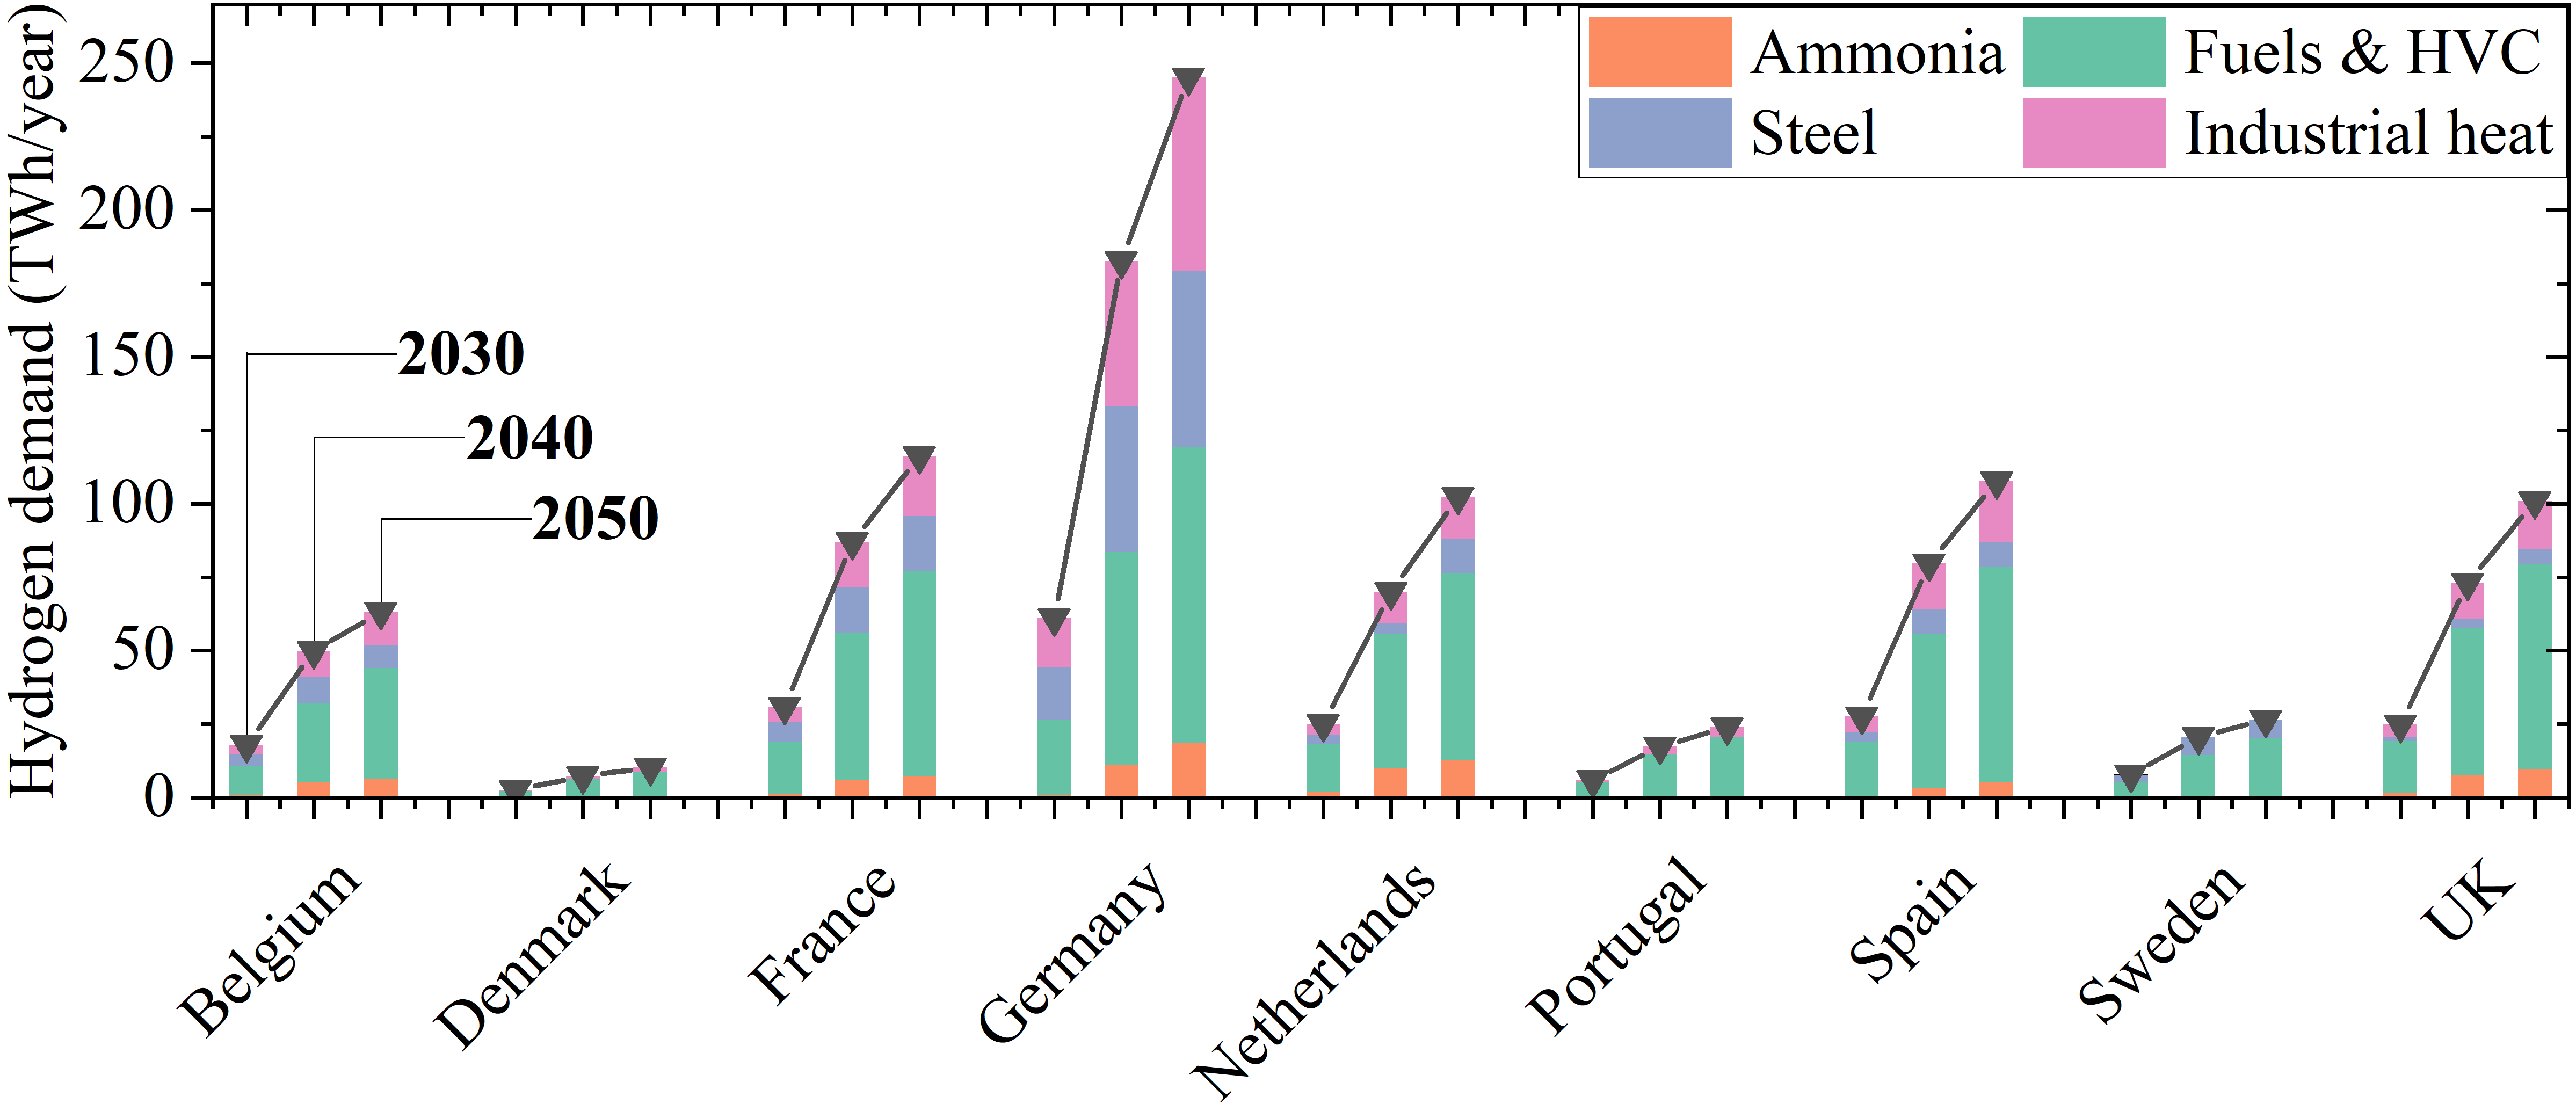
\includegraphics[width = 0.99\columnwidth]{figs/fighydrogendemand2.png}
    \caption{Hydrogen demand for coastal European countries}
    \label{fig hydrogen demand}
\end{figure}

\begin{table}[]
\centering
\caption{Offshore wind capacity in European countries}
\label{tab owf capacity}
\begin{tabular}{llll}
\hline
               & \multicolumn{3}{l}{Capacity   (GW)} \\ \hline
               & 2030       & 2040       & 2050      \\ \hline
Belgium        & 6 \cite{NSOG}       & 8 \cite{NSOG}         & 8 \cite{NSOG}         \\
Denmark        & 9 \cite{Offshorewindfarmstenderedtowards2030}          & 10 \cite{EnergyIslandintheNorthSea}        & 35 \cite{NSOG}       \\
France         & 18 \cite{FrancepassesRenewable}        & 20 (estimated)         & 40 \cite{Francecommitsto40}       \\
Germany        & 30 \cite{Morewindenergyatsea}        & 40 \cite{Morewindenergyatsea}        & 70 \cite{Morewindenergyatsea}       \\
Ireland        & 5 \cite{FutureFrameworkforOffshoreRenewableEnergy}         & 20 \cite{FutureFrameworkforOffshoreRenewableEnergy}        & 37 \cite{FutureFrameworkforOffshoreRenewableEnergy}       \\
Netherlands    & 21 \cite{Offshorewindenergy}       & 50 \cite{NetherlandsSets70GW}        & 70 \cite{NetherlandsSets70GW}        \\
Norway         & 3  \cite{300GWNorthSea}        & 22 \cite{ENERGYTRANSITIONNORWAY2023}        & 43 \cite{ENERGYTRANSITIONNORWAY2023}       \\
Portugal       & 10 \cite{Portugaltolaunch}        & 10 \cite{Atlantic}        & 10 \cite{Atlantic}       \\
Spain          & 3  \cite{Spainissuesplan}        & 10 (estimated)          & 17 \cite{Spainrepresents}        \\
Sweden         & 3  \cite{FinlandDenmarkSweden}        & 11 (estimated) \cite{Roadmap2040}         & 41 \cite{Offshorewinddevelopment}       \\
United Kingdom & 55  \cite{Offshorewindnetzero}       & 80 \cite{Offshorewindnetzero}        & 125 \cite{Offshorewindnetzero}      \\ \hline
\end{tabular}
\end{table}

The offshore wind capacity of each country is listed in the Table.\ref{tab owf capacity}. The reference for each value is given. Most of the numbers are obtained from the official offshore wind development plans from governments. For those countries without clear written plans, we use the numbers from the latest EU's non-binding agreement or the press release by their governments. Among the offshore wind capacities, we assume half of them are equipped with electrolysers and can produce hydrogen, and 10\% can be used for ammonia production. These capacities set the upper limits of the total hydrogen and ammonia production capacity in a country. The annual domestic hydrogen consumption is calculated in the last section as $\sum_{i \in \mathcal{I}^E} \sum_{g \in \mathcal{G}^{ptg}} \sum_{h=1}^{8760} Q_{i,g,h}^{hy}$. Then, the available hydrogen export capacity $Q_{ic}^{hy,ex,max}$ can be calculated as:
\begin{align}
    Q_{ic}^{hy,ex,max} = 0.5 P_{ic}^{owf,max}  CF_{ic} \eta^{ptg}
\end{align}
where $P_{ic}^{owf,max}$ is the total offshore wind capacity for country $ic$, as can be obtained from Table. \ref{tab owf capacity}; $CF_{ic}$ is the average capacity factor for country $ic$.

\subsection{Domestic absorption sensitivity}

The main manuscript uses the hourly Ireland power-gas optimisation to estimate how much offshore production can be absorbed domestically, then scales the resulting domestic absorption by country-level electricity and gas demand before applying country export limits in the European trade model. To test whether this extrapolation drives the strategic-exporter conclusion, we multiply the domestic absorption estimate by 0.75 and 1.25 and resolve the integrated trade model. A lower factor means less domestic absorption and therefore more available export potential; a higher factor means more domestic absorption and therefore less available export potential.

\begin{table}[h]
\centering
\tiny
\setlength{\tabcolsep}{1pt}
\caption{Sensitivity of integrated trade results to domestic absorption scaling. Export potential (Export pot.), European offshore supply (Offshore), external imports (Import), Ireland net exports (IE net) and UK net exports (UK net) are reported in TWh yr$^{-1}$.}
\label{tab:domestic-absorption-sensitivity}
\begin{tabular}{llrrrrrr}
\hline
Year & Case & Factor & Export pot. & Offshore & Import & IE net & UK net \\ \hline
2030 & Low & 0.75 & 328 & 213 & 0 & 17 & 61 \\
2030 & Base & 1.00 & 287 & 213 & 0 & 14 & 78 \\
2030 & High & 1.25 & 248 & 214 & 0 & 12 & 98 \\
2040 & Low & 0.75 & 610 & 610 & 4 & 86 & 178 \\
2040 & Base & 1.00 & 495 & 495 & 116 & 83 & 122 \\
2040 & High & 1.25 & 380 & 380 & 229 & 78 & 66 \\
2050 & Low & 0.75 & 1003 & 830 & 0 & 142 & 227 \\
2050 & Base & 1.00 & 767 & 767 & 62 & 162 & 162 \\
2050 & High & 1.25 & 571 & 571 & 254 & 155 & 63 \\ \hline
\end{tabular}
\end{table}

The sensitivity changes the amount of European offshore supply that can compete with external imports, but it does not restore the lowest-LCOH exporter geography. In 2050, lower domestic absorption strengthens the UK as the largest net exporter, while higher domestic absorption makes Ireland the largest net exporter. Under the base case the two countries are nearly tied, at about 162 TWh yr$^{-1}$ each. The exact UK/Ireland ordering is therefore sensitive to domestic absorption, but Ireland remains one of the leading exporters across the tested range, and the integrated model continues to differ from the LCOH-only baseline.

\subsection{Optimal international trading model}

The optimal international trading model determines the hydrogen flow among these European countries. The optimization objective is to minimize the total external cost ($C^{ex}$), including production cost ($C^{prod}$), transportation cost ($C^{trans}$), and international import (import from other distant countries/regions such as Africa, Australia) cost $C^{im}$ during international hydrogen/ammonia trading to achieve a global optimum.  
\begin{align}
    \min C^{ex} & = C^{prod} + C^{trans} + C^{im}
    \notag \\
    & = \sum_{ic \in \mathcal{CT}} f^{prod}\left(Q_{ic}^{hy,spl} 
    + Q_{ic}^{am,spl} \right) 
     + \sum_{ip \in \mathcal{PT}} \sum_{jp \in \mathcal{PT}}^{jp \neq ip} \left(C_{ip,jp}^{trans,hy} + C_{ip,jp}^{trans,am} \right) 
     \notag\\
     & + \rho^{im,hy} \sum_{ic \in \mathcal{CT}}Q_{ic}^{hy,im} + \rho^{im,am} \sum_{ic \in \mathcal{CT}}Q_{ic}^{am,im}
\end{align}
where $ic$ is the index for countries and $ip$, $jp$ are the indices for ports; $\mathcal{CT}$ and $\mathcal{PT}$ are the sets of countries and ports, respectively; $f^{prod}$ is the piecewise production cost function, fitted from the cost-supply curves in Section. \ref{sec cost}; $Q_{ic}^{hy,spl}$ and $Q_{ic}^{am,spl}$ are the hydrogen and ammonia production from country $ic$, respectively; $C_{ip,jp}^{trans,hy}$ is the total shipping cost in the shipping line that links port $ip$ and $jp$; $\rho^{im,hy}$ and $\rho^{im,am}$ are the unit costs for international import hydrogen and ammonia, respectively; $Q_{ic}^{hy,im}$ and $Q_{ic}^{am,im}$ are the quantities of import hydrogen and ammonia for country $ic$, respectively.

It subject to:

(1) Supply and demand constraints:

The offshore wind can supply electricity, hydrogen, and ammonia. The sum of hydrogen and ammonia productions should be within the available hydrogen production capacity, as in (\ref{eq offshore production hydrogen cons}). Similar for ammonia constraints (\ref{eq offshore production ammonia cons}). (\ref{eq country hydrogen balance cons}) and (\ref{eq country ammonia balance cons}) model the supply-demand balance for hydrogen and ammonia in a country, respectively.
\begin{gather}
    0 \leq Q_{ic}^{hy,spl} + Q_{ic}^{am,spl} (\eta^{asr})^{-1} \leq Q_{ic}^{hy,ex,max}
\label{eq offshore production hydrogen cons}\\
    0 \leq Q_{ic}^{am,spl} \leq Q_{ic}^{am,ex,max}
\label{eq offshore production ammonia cons}\\
    Q_{ic}^{hy,spl} - \sum_{ip \in \mathcal{PT}_{ic}} \sum_{jp \in \mathcal{PT}}^{jp \notin \mathcal{PT}_{ic}} \left( Q_{ip,jp}^{hy,trans} + Q_{ip,jp}^{hy,route} \right) - Q_{ic}^{hy,dm} + Q_{ic}^{hy,im}= 0
\label{eq country hydrogen balance cons}\\
    Q_{ic}^{am,spl} - \sum_{ip \in \mathcal{PT}_{ic}} \sum_{jp \in \mathcal{PT}}^{jp \notin \mathcal{PT}_{ic}} \left( Q_{ip,jp}^{am,trans} + Q_{ip,jp}^{am,route} \right) - Q_{ic}^{am,dm} + Q_{ic}^{am,im}  = 0
\label{eq country ammonia balance cons}
\end{gather}
where $\eta^{asr}$ is the efficiency of the ammonia synthesis reactor; $Q_{ic}^{am,ex,max}$ is the export capacity of ammonia for country $ic$; $\mathcal{PT}_{ic}$ is the set of ports located in the country $ic$; $Q_{ip,jp}^{hy,trans}$ and $Q_{ip,jp}^{am,trans}$ are the annual hydrogen and ammonia shipped from port $ip$ to $jp$, respectively; $Q_{ip,jp}^{hy,route}$ and $Q_{ip,jp}^{am,route}$ are the annual fuel (hydrogen or ammonia) consumptions of all ships operating on the route between port $ip$ and $jp$, respectively; $Q_{ic}^{hy,dm}$ and $Q_{ic}^{am,dm}$ are the domestic hydrogen and ammonia for country $ic$, respectively.

(2) Transportation costs and constraints:

The transportation cost for a shipping line consists of labour costs and fuel costs. For a specific ship, given the annual operation days ($T^{op}$), the number of trips in a year ($n^{trip}$) can be calculated as:
\begin{gather}
    n_{ip,jp}^{trip} = \frac{T^{op}}{2(T_{ip,jp}^{tv} + T^{ld})}
\\
    T_{ip,jp}^{tv} = L_{ip,jp} / v^{ship}
\end{gather}
where $T_{ip,jp}^{tv}$ and $T^{ld}$ are the travelling time and load/unload time; $L_{ip,jp}$ is the distance long the shipping line between port $ip$ and $jp$; $v^{ship}$ is the velocity of ships.

The country-wide average unit fuel cost of shipping hydrogen is shown in Fig. \ref{fig ship cost}. The cost depends on the shipping routes' lengths, which can be obtained from SeaRates \cite{SEAPATES}. Considering the around 60 €/MWh marginal price for hydrogen, the transportation fuel cost accounts for around 0.08\% - 2.12\%. From Fig. \ref{fig ship cost}. a to Fig. \ref{fig ship cost}.c, the fuel cost will generally decline due to the reduced cost of hydrogen. Among different shipping routes, the ones connected to Portugal, such as Sweden and Norway, have relatively higher costs due to the distant locations.

\begin{figure}
    \centering
    
\includegraphics[width = 0.5\columnwidth]{figs/fig shipping fuel cost.pdf}
    \caption{Fuel cost for shipping liquid hydrogen}
    \label{fig ship cost}
\end{figure}


Then, the total capacity per year of a port-to-port shipping line, and its fuel consumption can be calculated as:
\begin{gather}
    Q_{ip,jp}^{hy,trans,max} = Q_{ip,jp}^{hy,ship,max} n_{ip,jp}^{trip} n_{ip,jp}^{hy,ship}
\label{eq hy ship flow} \\
    Q_{ip,jp}^{am,trans,max} = Q_{ip,jp}^{am,ship,max} n_{ip,jp}^{trip} n_{ip,jp}^{am,ship}
\label{eq am ship flow} \\
    Q_{ip,jp}^{hy,trans} \leq  Q_{ip,jp}^{hy,trans,max}
\label{eq hy ship cap} \\
    Q_{ip,jp}^{am,trans} \leq  Q_{ip,jp}^{am,trans,max}
\label{eq am ship cap} \\
    Q_{ip,jp}^{hy,route} = 2 n_{ip,jp}^{trip} T_{ip,jp}^{tv} Q^{hy,ship}
\label{eq hy ship fuel} \\
    Q_{ip,jp}^{am,route} = 2 n_{ip,jp}^{trip} T_{ip,jp}^{tv} Q^{am,ship}
\label{eq am ship fuel}
\end{gather}
where $Q_{ip,jp}^{hy,trans,max}$ and $Q_{ip,jp}^{am,trans,max}$ are the maximum hydrogen and ammonia transportation capacities between port $ip$ and $jp$, respectively; $Q_{ip,jp}^{hy,ship,max}$ and $Q_{ip,jp}^{am,ship,max}$ are the hydrogen and ammonia storage capacities per ship, respectively; $n_{ip,jp}^{hy,ship}$ and $n_{ip,jp}^{am,ship}$ are the numbers of invested hydrogen and ammonia transportation ships between port $ip$ and $jp$, respectively; they are the decision variables in the optimisation problem; $Q^{hy,ship}$ and $Q^{am,ship}$ are the operating hydrogen and ammonia fuel consumptions per ship per hour, respectively.

Then, the annual cost for year $t$ of the shipping line can be summed up as:
\begin{align}
    C_{ip,jp}^{trans,hy} =  n_{ip,jp}^{hy,ship} \left( \frac{C^{cap,ship}}{\sum_{t = 0}^{t = T^{ship}-1} (1+r)^{t-1}} + C^{om,ship} \right)
    \\
    C_{ip,jp}^{trans,am} =  n_{ip,jp}^{am,ship} \left( \frac{C^{cap,ship}}{\sum_{t = 0}^{t = T^{ship}-1} (1+r)^{t-1}} + C^{om,ship} \right)
\end{align}
where $C^{cap,ship}$ and $C^{om,ship}$ are the capital cost and annual operation and maintenance cost, respectively; $T^{ship}$ is the lifespan of the ship.
The transportation cost of ammonia ($C_{ip,jp}^{trans,am}$) can be calculated similarly.

(3) Solution method

Due to the discontinuity of the hydrogen and ammonia cost-supply curves, the original problem is formulated as a mixed integer linear programming problem, and is solved by Gurobi \cite{Gurobi} commercial solver via the Yalmip modelling toolbox in Matlab.

\subsection{Carbon-mitigation accounting}

After solving the international trading model, carbon mitigation is reported as a direct displacement-accounting metric rather than a full lifecycle assessment. Hydrogen and ammonia quantities are represented in the optimisation as average delivered power $Q$ in MW, so annual delivered energy is $Q \times 8760 \times 3600$ MJ yr$^{-1}$. For demand country $ic$, the model reports:
\begin{align}
    M_{ic}^{hy} &= Q_{ic}^{hy,dm} \frac{8760 \times 3600}{H^{ng}}\frac{44}{16}\frac{1}{10^9},\\
    M_{ic}^{am} &= Q_{ic}^{am,dm} \frac{8760 \times 3600}{H^{am}}\frac{44}{17}\frac{1}{10^9},\\
    M_{ic} &= M_{ic}^{hy} + M_{ic}^{am},
\end{align}
where $M_{ic}$ is in Mt CO$_2$ yr$^{-1}$, $H^{ng}=50$ MJ kg$^{-1}$ is the natural-gas lower heating value used for the hydrogen-demand displacement term, and $H^{am}=23$ MJ kg$^{-1}$ is the ammonia lower heating value used for the ammonia-demand displacement term. The factors 44/16 and 44/17 convert methane and ammonia mass-equivalent terms to CO$_2$ mass-equivalent terms in the model accounting.

The supplier contribution matrix applies the same conversion to optimized hydrogen and ammonia deliveries between each supplier and demand country. If a positive flow is sent from supplier $ic$ to demand country $jc$, the corresponding avoided CO$_2$ is assigned to matrix element $A_{ic,jc}$. If the optimized route variable is negative, the direction is reversed before assignment. External imports are assigned to an additional international-import row, labelled ITN in the Sankey figure. Domestic self-supply is assigned on the diagonal as the residual demand-country mitigation after imported contributions are subtracted:
\begin{align}
    A_{ic,ic} = M_{ic} - \sum_{r \neq ic} A_{r,ic}.
\end{align}
The total carbon mitigation reported in the main text is $\sum_r \sum_{ic} A_{r,ic}$. The European offshore supplier contribution excludes the ITN row and is therefore smaller than the total whenever external imports contribute to meeting demand.

\begin{table}[h]
\centering
\caption{Carbon-mitigation accounting values used in the main manuscript. Total mitigation includes the external import node when present. European offshore contribution excludes the external import node.}
\label{tab carbon accounting summary}
\begin{tabular}{lrrr}
\hline
Metric & 2030 & 2040 & 2050 \\ \hline
Total mitigation (Mt CO$_2$ yr$^{-1}$) & 43.5 & 129.8 & 175.5 \\
European offshore contribution (Mt CO$_2$ yr$^{-1}$) & 43.5 & 103.2 & 158.3 \\
External import (TWh yr$^{-1}$) & 0.0 & 116.2 & 62.2 \\ \hline
\end{tabular}
\end{table}





%%===========================================================================================%%
%% If you are submitting to one of the Nature Portfolio journals, using the eJP submission   %%
%% system, please include the references within the manuscript file itself. You may do this  %%
%% by copying the reference list from your .bbl file, paste it into the main manuscript .tex %%
%% file, and delete the associated \verb+\bibliography+ commands.                            %%
%%===========================================================================================%%

\bibliography{sn-bibliography}% common bib file
%% if required, the content of .bbl file can be included here once bbl is generated
%%\input sn-article.bbl


\end{document}
